\documentclass[onecolumn,12pt,a4paper]{IEEEtran}
\usepackage[utf8]{inputenc}
\usepackage[T1]{fontenc}
\usepackage[spanish]{babel}
\usepackage{cite,graphicx,booktabs,longtable,array,hyperref,tikz}
\AtBeginDocument{\spanishplainpercent}
\usetikzlibrary{shapes,arrows.meta,positioning}

\hypersetup{hidelinks}
\setlength{\emergencystretch}{3em}
\renewcommand{\thesection}{\arabic{section}}
\renewcommand{\thesubsection}{\thesection.\arabic{subsection}}
\renewcommand{\thesubsubsection}{\thesubsection.\arabic{subsubsection}}
\renewcommand{\tablename}{Tabla}
\renewcommand{\figurename}{Figura}
\newif\ifCincoConclusiones
\CincoConclusionestrue

\begin{document}
\nocite{iso29148,iso15288,iso12207,iso25010,pohl2025,swebok4,pmbok7,ireb2023,moore,mavin2009}

\begin{titlepage}
\centering
\vfill
{\fontsize{14}{16}\selectfont\textbf{UNIVERSIDAD TÉCNICA ESTATAL DE QUEVEDO}}\par
\vspace{0.45cm}

\includegraphics[width=0.15\textwidth]{figura/LogoUTEQ.jpg}\par
\vspace{0.35cm}
{\fontsize{14}{16}\selectfont\textbf{FACULTAD DE CIENCIAS DE LA COMPUTACIÓN}}\par
{\fontsize{13}{15}\selectfont\textbf{CARRERA DE INGENIERÍA EN SOFTWARE}}\par
\vspace{0.6cm}
{\fontsize{14}{16}\selectfont\textbf{TEMA:}}\par
{\fontsize{12}{15}\selectfont GA-PE-U · SUM · Práctica Experimental Unidad I}\par\vspace{0.35cm}
{\fontsize{14}{16}\selectfont\textbf{ASIGNATURA:}}\par
{\fontsize{12}{14}\selectfont INGENIERÍA DE REQUERIMIENTOS}\par
\vspace{0.35cm}
{\fontsize{14}{16}\selectfont\textbf{DOCENTE:}}\par
{\fontsize{12}{14}\selectfont ING. GUERRERO ULLOA GLEISTON CICERÓN}\par
\vspace{0.35cm}
{\fontsize{14}{16}\selectfont\textbf{INTEGRANTES:}}\par
{\fontsize{11.5}{14}\selectfont MENDOZA PALMA ALLAN JEREMY, CI: 0956082309, amendozap10@uteq.edu.ec -- Analista líder, documentador y investigador A}\par
{\fontsize{11.5}{14}\selectfont ROCHINA ROCHINA FREDDY DAVID, CI: 0250214103, frochinar@uteq.edu.ec -- Investigador B}\par
{\fontsize{11.5}{14}\selectfont SÁNCHEZ CENTENO ROSELYN ANDREINA, CI: 1250178876, rsanchezc4@uteq.edu.ec -- Investigadora C}\par
\vspace{0.35cm}
{\fontsize{14}{16}\selectfont\textbf{EQUIPO:}}\par
{\fontsize{12}{14}\selectfont MRS}\par
\vspace{0.25cm}
{\fontsize{14}{16}\selectfont\textbf{CURSO/PARALELO:}}\par
{\fontsize{12}{14}\selectfont CUARTO NIVEL, PARALELO ``B''}\par
\vspace{0.25cm}
{\fontsize{14}{16}\selectfont\textbf{SISTEMA PFC:}}\par
{\fontsize{12}{14}\selectfont Plataforma de ventas con módulo de recomendación basado en IA para el soporte de ventas en establecimientos eléctricos}\par
\vspace{0.25cm}
{\fontsize{14}{16}\selectfont \textbf{REPOSITORIO PE4:}}\\
{\fontsize{12}{14}\selectfont \url{https://github.com/AllanMendoza09/IR-trabajos-grupales-MRS.git}}\\[0.3cm]
{\fontsize{14}{16}\selectfont\textbf{SEMANA DE ENTREGA:}}\par
{\fontsize{12}{14}\selectfont SEMANA 3}\par
\vspace{0.45cm}
{\fontsize{14}{16}\selectfont\textbf{QUEVEDO -- LOS RÍOS -- ECUADOR}}\par
{\fontsize{14}{16}\selectfont\textbf{2026 -- 2027 SPA}}\par
\vfill
\end{titlepage}

\tableofcontents
\clearpage

\section*{0. Sistema del PFC: descripción inicial y partes interesadas}

\addcontentsline{toc}{section}{0. Sistema del Proyecto Fin de Curso}

\textbf{Descripción del sistema.} La «Plataforma de ventas con módulo de recomendación basado en IA para el soporte de ventas en establecimientos eléctricos» se propone para locales comerciales de Quevedo, Ecuador. Su propósito es apoyar el registro de ventas, la consulta de existencias y la atención técnica al cliente. Actualmente se reportan dificultades asociadas con facturación lenta, interfaces poco prácticas, datos mal administrados y errores de digitación, especialmente durante horas de alta demanda. Además, los cajeros dependen de trabajadores experimentados para responder consultas sobre productos eléctricos. Los usuarios previstos son cajeros, administradores, propietarios, clientes y auditores; los proveedores y servicios de pago forman parte del contexto externo. Se considera una aplicación web con PostgreSQL y un servicio externo de modelos de lenguaje mediante Groq. Estas decisiones son preliminares y requieren confirmación con el establecimiento.

\noindent\textbf{Mapa conceptual integrador (Paso 5d).} La Figura~\ref{fig:mapa_conceptual} sintetiza los cuatro temas de la Unidad 1 y los vincula con el PFC. Los vínculos cruzados relacionan el proceso con la clasificación, la clasificación con las propiedades de calidad, y la participación de los actores con la validación \cite{pohl2025,iso29148,ireb2023}.

\begin{figure}[!htbp]
\centering
\IfFileExists{figura/mapa_conceptual.pdf}{
  \includegraphics[width=\linewidth,height=0.35\textheight,keepaspectratio]{figura/mapa_conceptual.pdf}
}{
  \fbox{\parbox[c][5cm][c]{0.93\linewidth}{\centering Mapa conceptual integrador (Paso 5d).\\
  Exportar desde diagrams.net como \texttt{figura/mapa\_conceptual.pdf}.}}
}
\caption{Mapa conceptual integrador de la Unidad 1 y su aplicación al PFC (Paso 5d).}
\label{fig:mapa_conceptual}
\end{figure}

\textbf{Matriz poder/interés.} El análisis de partes interesadas relaciona su capacidad de influir en decisiones y el nivel de atención que prestan a los resultados del proyecto \cite{pmbok7}. La Figura~\ref{fig:poderinteres} presenta una distribución inicial, mientras que la Tabla~\ref{tab:stakeholders} documenta sus criterios de gestión. Se trata de una clasificación argumentada por el equipo, no de una encuesta realizada.

\begin{figure}[htbp]
\centering
\begin{tikzpicture}[x=1cm,y=1cm,font=\small]
\draw[thick] (0,0) rectangle (13,7);
\draw[thick] (6.5,0)--(6.5,7);
\draw[thick] (0,3.5)--(13,3.5);
\node[font=\bfseries] at (3.25,6.5) {Mantener informados};
\node[font=\bfseries] at (9.75,6.5) {Gestionar de cerca};
\node[font=\bfseries] at (3.25,3.05) {Monitorear};
\node[font=\bfseries] at (9.75,3.05) {Mantener satisfechos};
\node[draw,rounded corners,fill=white,align=center] at (9.6,5.5) {Propietario};
\node[draw,rounded corners,fill=white,align=center] at (9.6,4.45) {Administrador};
\node[draw,rounded corners,fill=white,align=center] at (3.15,5.5) {Cajeros};
\node[draw,rounded corners,fill=white,align=center] at (3.15,4.45) {Clientes};
\node[draw,rounded corners,fill=white,align=center] at (9.6,1.55) {Auditor};
\draw[-{Stealth},thick] (0,-0.42)--(13,-0.42) node[right]{Poder};
\node[below] at (0,-0.42) {Bajo};
\node[below] at (13,-0.42) {Alto};
\draw[-{Stealth},thick] (-0.42,0)--(-0.42,7) node[above]{Interés};
\node[left] at (-0.42,0) {Bajo};
\node[left] at (-0.42,7) {Alto};
\end{tikzpicture}
\caption{Matriz poder/interés propuesta para los cinco stakeholders iniciales del PFC.}
\label{fig:poderinteres}
\end{figure}

\small
\begin{longtable}{@{}p{2.3cm}p{1.0cm}p{1.0cm}p{2.3cm}p{3.0cm}p{4.6cm}@{}}
\caption{Clasificación preliminar y estrategias de gestión de stakeholders.}\label{tab:stakeholders}\\
\toprule
\textbf{Actor} & \textbf{Poder} & \textbf{Interés} & \textbf{Cuadrante} & \textbf{Estrategia} & \textbf{Justificación provisional}\\\midrule
\endfirsthead
\toprule
\textbf{Actor} & \textbf{Poder} & \textbf{Interés} & \textbf{Cuadrante} & \textbf{Estrategia} & \textbf{Justificación provisional}\\\midrule
\endhead
Propietario & Alto & Alto & Gestionar de cerca & Revisar alcance y prioridades & Decide sobre inversión y necesita mejorar ventas y atención.\\
Administrador & Alto & Alto & Gestionar de cerca & Talleres y aprobación operativa & Define autorizaciones, inventario y reglas diarias.\\
Cajeros & Bajo & Alto & Mantener informados & Entrevistas y prototipos & Operan ventas y enfrentan errores de digitación.\\
Clientes & Bajo & Alto & Mantener informados & Pruebas de tareas y retroalimentación & Reciben asesoría y comprobantes; afectan la aceptación del servicio.\\
Auditor & Alto & Bajo & Mantener satisfechos & Revisiones de registros y controles & Puede exigir evidencias de trazabilidad, aunque no opera cada venta.\\
\bottomrule
\end{longtable}
\normalsize

\textbf{Clasificación provisional del sistema.} La propuesta se clasifica como \emph{sistema software-intensivo de información transaccional para ventas e inventario, con un componente de recomendación basado en IA}. Los procesos de venta, consulta de existencias y control de artículos tratan información comercial y registran transacciones que deben conservar integridad. En una perspectiva de ingeniería de sistemas, el servicio interactúa con personas, dispositivos de atención, una base de datos y proveedores externos; estas interacciones justifican analizar el ciclo de vida del sistema y sus interfaces \cite{iso15288,pohl2025}. La clasificación es funcional, no una declaración de arquitectura ya validada.

Además, el componente transaccional y el módulo de recomendación son dependencias de software que deberán diseñarse, probarse y mantenerse durante la operación \cite{iso12207,iso15288}. PostgreSQL y Groq se consideran alternativas tecnológicas iniciales, sujetas a restricciones de costo, conectividad, datos personales y disponibilidad. El componente de recomendación debe apoyar al cajero sin sustituir una comprobación técnica cuando exista riesgo de uso incorrecto de material eléctrico. El límite del sistema y las ocho perspectivas de contexto se desarrollan en las secciones 3.7 y 3.9, respectivamente; la clasificación queda unificada para todo el informe.

\setcounter{section}{1}
\section{Fundamento teórico}

\subsection{Fundamentos de la Ingeniería de Requisitos}

\textbf{Ingeniería de Requisitos (IR).} \emph{Definición parafraseada:} disciplina sistemática que permite descubrir, analizar, documentar, comprobar y mantener las necesidades y restricciones que debe satisfacer un sistema \cite{iso29148,pohl2025}. \emph{Explicación:} Su trabajo inicia antes de programar porque primero debe identificarse el problema correcto. Requiere dialogar con usuarios que pueden tener necesidades diferentes y registrar acuerdos comprobables. También continúa cuando el sistema evoluciona, debido a cambios operativos y normativos. \emph{Ejemplo:} antes de construir una pantalla de cobro, se investiga por qué los cajeros se equivocan al digitar códigos o precios.

\textbf{Requisito.} \emph{Definición parafraseada:} condición o capacidad necesaria para satisfacer una necesidad de una parte interesada o una obligación, cuya expresión documentada sirve para especificación y verificación \cite{iso29148,pohl2025}. \emph{Explicación:} Un requisito no es simplemente el nombre de una función. Debe expresar un comportamiento o condición identificable y permitir comprobar si se cumplió. Cuando carece de precisión, dos implementadores pueden interpretar resultados distintos. \emph{Ejemplo:} «registrar una venta con detalle y un identificador único al confirmarse el cobro» es más verificable que «mejorar las ventas».

\textbf{Objetivos y principios de la IR.} \emph{Definición parafraseada:} son criterios para obtener acuerdos suficientes, representar necesidades correctas y producir requisitos comprensibles, consistentes y verificables \cite{pohl2025,ireb2023,iso29148}. \emph{Explicación:} El objetivo no es maximizar la cantidad de requisitos, sino eliminar incertidumbre importante. Los acuerdos deben negociarse cuando una necesidad de rapidez entra en conflicto con controles de seguridad. La expresión «no funcional» también requiere precisión conceptual para evitar especificaciones ininterpretables \cite{glinz2007}. La trazabilidad ayuda a saber qué necesidad explica cada requisito. \emph{Ejemplo:} el propietario busca reducir tiempos de cobro, pero el auditor necesita rastrear quién anuló una venta.

\textbf{Defectos y costo de las omisiones.} \emph{Definición parafraseada:} un defecto de requisito es una deficiencia como ambigüedad, omisión o contradicción que impide interpretarlo o utilizarlo con confianza \cite{iso29148,wiegers2013}. \emph{Explicación:} Detectar un error antes del desarrollo permite corregir un texto o una regla de negocio. Si se descubre después de programar, puede ser necesario modificar pantallas, operaciones y pruebas. No se asigna un multiplicador de costos, porque no se dispone de una medición específica para este PFC. \emph{Ejemplo:} omitir reglas de devolución obliga a rehacer el flujo de caja si el negocio trabaja con notas de crédito.

\textbf{Relación con los ciclos de vida.} \emph{Definición parafraseada:} los marcos de ciclo de vida organizan los procesos aplicables al sistema y al software desde su concepción hasta su retiro \cite{iso15288,iso12207}. \emph{Explicación:} La IR aporta una base para el diseño y las pruebas, pero también recibe cambios desde la operación. SWEBOK v4.0 organiza la Ingeniería de Requisitos como un área del conocimiento de ingeniería de software \cite{swebok4}. Por eso, los requisitos deben mantenerse coherentes entre versiones, no quedar congelados sin revisión. \emph{Ejemplo:} cuando el establecimiento incorpore un nuevo método de pago, habrá que revisar requisitos de integración y auditoría.

\subsection{Proceso de Ingeniería de Requisitos}

\textbf{Proceso de IR.} \emph{Definición parafraseada:} conjunto organizado y adaptable de actividades y productos de trabajo que permite desarrollar y mantener requisitos acordados durante la vida del sistema \cite{pohl2025,swebok4,ireb2023}. \emph{Explicación:} No existe una única secuencia rígida adecuada para todos los proyectos. En esta plataforma, una entrevista puede llevar a un prototipo y luego a nuevas preguntas. El proceso deberá repetirse al descubrir excepciones comerciales. \emph{Ejemplo:} una observación de ventas con descuentos puede originar un nuevo candidato a requisito.

\textbf{Elicitación.} \emph{Definición parafraseada:} actividad de identificar fuentes y obtener necesidades y conocimiento del contexto mediante interacción o análisis de evidencia \cite{pohl2025,ireb2023}. \emph{Explicación:} Las opiniones del propietario no reemplazan la observación de los cajeros. Cada técnica revela problemas distintos y requiere registrar su procedencia. La entrevista obtiene explicaciones y la observación permite detectar pasos que el usuario omite al narrarlos. \emph{Ejemplo:} registrar cómo se localiza un interruptor cuando su código no está visible.

\textbf{Análisis y negociación.} \emph{Definición parafraseada:} estudio de requisitos candidatos para detectar conflictos, dependencias, defectos y alternativas que requieren acuerdo entre interesados \cite{pohl2025,ireb2023}. \emph{Explicación:} Una necesidad puede afectar a otras y debe evaluarse antes de aprobarse. Las prioridades del propietario no siempre coinciden con las del cajero o auditor. La negociación documenta una decisión en lugar de ocultar discrepancias. \emph{Ejemplo:} discutir si se permitirá vender un producto con stock negativo.

\textbf{Especificación y documentación.} \emph{Definición parafraseada:} representación organizada de los requisitos mediante texto, modelos o estructuras que permitan compartir y revisar acuerdos \cite{iso29148,pohl2025}. \emph{Explicación:} Los requisitos deben usar términos consistentes como «venta», «artículo» y «comprobante». Se necesita un identificador que facilite vincularlos con evidencia y pruebas. Las plantillas de lenguaje controlado ayudan a reducir ambigüedades \cite{mavin2009}. \emph{Ejemplo:} especificar en un requisito cuándo se registra una operación de caja y qué datos persisten.

\textbf{Validación.} \emph{Definición parafraseada:} evaluación de los requisitos para comprobar que expresan las necesidades y restricciones correctas de las partes interesadas \cite{pohl2025,iso29148}. \emph{Explicación:} Una revisión de texto permite encontrar defectos, pero no confirma por sí sola que el negocio está de acuerdo. Para lograr esa confirmación deben participar representantes con capacidad de aprobar reglas. En esta fase solo se realizará revisión documental de tres ejemplos; no se afirmará aceptación del local. \emph{Ejemplo:} contrastar con un cajero si el flujo de registro propuesto corresponde a una venta real.

\textbf{Gestión, trazabilidad y línea base.} \emph{Definición parafraseada:} prácticas que identifican versiones de requisitos, mantienen sus relaciones y controlan modificaciones después de establecer un conjunto aprobado \cite{pohl2025,iso29148,ireb2023,hull2011}. \emph{Explicación:} La trazabilidad permite seguir un requisito desde su necesidad hasta su prueba. La línea base establece un punto de referencia sometido a control formal de cambios. Una solicitud de modificación debe analizar impacto antes de incorporarse al conjunto aprobado. \emph{Ejemplo:} cambiar la regla de descuentos obliga a revisar cálculo del total, comprobante, permisos y pruebas asociadas.

	\subsection{Tipos de requisitos}

	La clasificaci\'on sistem\'atica de los requisitos permite estructurar las necesidades del negocio y traducirlas en especificaciones t\'ecnicas verificables a lo largo del ciclo de vida del sistema \cite{iso29148,iso15288,iso12207}. De acuerdo con Pohl \cite{pohl2025} y Glinz \cite{glinz2007}, la clasificaci\'on fundamental distingue tres categor\'ias principales: los requisitos funcionales, los requisitos de calidad y las restricciones. Esta distinci\'on evita mezclar comportamientos operativos con atributos de desempe\~no o limitaciones arquitect\'onicas \cite{pohl2025,glinz2007}. Por su parte, la norma ISO/IEC/IEEE 29148:2018 establece una jerarqu\'ia desde el nivel organizacional hasta el detalle t\'ecnico del sistema \cite{iso29148}.

	\textbf{Requisitos de negocio.} Definici\'on formal: declaraciones de alto nivel que expresan las metas, objetivos estrat\'egicos y beneficios esperados por la organizaci\'on que patrocina el sistema \cite{iso29148,wiegers2013}. Explicaci\'on propia: Estos requisitos justifican la inversi\'on econ\'omica y orientan el alcance general del proyecto sin detallar mecanismos t\'ecnicos de implementaci\'on. Su cumplimiento se mide mediante indicadores comerciales como reducci\'on de costos, incremento de ventas o disminuci\'on de tiempos operativos. Si un requisito funcional no contribuye a un objetivo de negocio, su inclusi\'on en el alcance debe cuestionarse. Ejemplo en el PFC: reducir los errores de digitaci\'on en el mostrador durante las horas pico para evitar p\'erdidas econ\'omicas y retrasos en la atenci\'on del local el\'ectrico en Quevedo.

	\textbf{Requisitos de partes interesadas (stakeholder).} Definici\'on formal: necesidades, expectativas y condiciones expresadas por los individuos u organizaciones que tienen un inter\'es leg\'itimo o se ven afectados por el sistema \cite{iso29148,pmbok7}. Explicaci\'on propia: Cada actor observa el problema desde su propia responsabilidad operativa, por lo que sus expectativas suelen entrar en conflicto y requieren negociaci\'on. Documentarlos permite mantener la trazabilidad entre qui\'en solicita una capacidad y c\'omo se resuelve en el software. Ignorar a un actor clave provoca rechazo durante la implantaci\'on o incumplimientos de control interno. Ejemplo en el PFC: el auditor exige conservar registros inalterables de cada anulaci\'on de venta, mientras el propietario demanda agilidad en el cierre diario de caja.

	\textbf{Requisitos de usuario.} Definici\'on formal: descripci\'on de las tareas, objetivos operativos y resultados que los usuarios finales deben poder ejecutar mediante el sistema en su entorno de trabajo \cite{iso29148,ireb2023}. Explicaci\'on propia: Se redactan desde la perspectiva del operador directo utilizando vocabulario del dominio comercial y evitando jerga de programaci\'on. Sirven como puente entre las expectativas generales de los interesados y las especificaciones detalladas del software. Su correcta formulaci\'on facilita la validaci\'on temprana mediante prototipos de interfaz. Ejemplo en el PFC: un cajero debe poder localizar un interruptor termomagn\'etico por descripci\'on parcial o amperaje cuando el cliente desconoce el c\'odigo exacto del fabricante.

	\textbf{Requisitos de sistema.} Definici\'on formal: especificaciones t\'ecnicas que definen las capacidades, caracter\'isticas y condiciones que el sistema completo (software, hardware y procedimientos) debe satisfacer para cumplir los requisitos de usuario \cite{iso29148,iso15288}. Explicaci\'on propia: Representan la vista externa e interna del producto que el equipo de ingenier\'ia dise\~nar\'a, construir\'a y verificar\'a. A diferencia de los requisitos de usuario, incorporan condiciones de frontera, manejo de excepciones y estados operativos precisos. Constituyen la base contractual y t\'ecnica para las pruebas de integraci\'on y aceptaci\'on. Ejemplo en el PFC: el sistema deber\'a registrar la venta y descontar existencias en una transacci\'on de base de datos, gestionando la impresi\'on como operaci\'on independiente susceptible de reintento.

	\textbf{Requisitos funcionales (RF).} Definici\'on formal: especificaciones que definen las acciones, transformaciones de datos y comportamientos observables que el sistema debe ejecutar ante entradas o eventos determinados \cite{iso29148,pohl2025,swebok4}. Explicaci\'on propia: Responden a la pregunta de qu\'e debe hacer el software para aportar valor operativo a sus usuarios. Para evitar ambig\"uedades en su redacci\'on, la literatura recomienda emplear plantillas de sintaxis controlada como el enfoque EARS \cite{mavin2009}. Cada funci\'on especificada debe ser comprobable mediante casos de prueba de caja negra. Ejemplo en el PFC: cuando el cajero ingresa la tensi\'on nominal y la potencia de carga solicitada por un cliente, el m\'odulo de recomendaci\'on debe desplegar hasta tres productos compatibles del cat\'alogo.

	\textbf{Requisitos no funcionales (RNF) o de calidad.} Definici\'on formal: atributos y propiedades que califican el grado en que el sistema ejecuta sus funciones, abarcando caracter\'isticas definidas en el modelo de calidad del producto software ISO/IEC 25010:2023 \cite{iso25010,pohl2025,glinz2007}. Explicaci\'on propia: Mientras los requisitos funcionales establecen la conducta del sistema, los de calidad determinan qu\'e tan bien, seguro, usable o fiable resulta dicho comportamiento. Seg\'un ISO/IEC 25010:2023, la calidad del producto se eval\'ua mediante caracter\'isticas como adecuaci\'on funcional, eficiencia de desempe\~no, compatibilidad, capacidad de interacci\'on (usabilidad), fiabilidad, seguridad, mantenibilidad y flexibilidad (portabilidad) \cite{iso25010}.
	Para ser verificables, todo RNF debe expresarse con una m\'etrica cuantificable y un umbral objetivo. Ejemplo en el PFC: un cajero nuevo debe completar una factura de cinco art\'iculos sin asistencia externa tras una capacitaci\'on m\'axima de treinta minutos.

	\textbf{Requisitos de rendimiento.} Definici\'on formal: subcategor\'ia de los requisitos de calidad que especifica las restricciones cuantitativas sobre velocidad de respuesta, capacidad de procesamiento, uso de recursos y concurrencia del sistema \cite{iso29148,iso25010,wiegers2013}. Explicaci\'on propia: Son cr\'iticos en entornos transaccionales donde la lentitud de respuesta deteriora directamente la experiencia de atenci\'on al p\'ublico. Su especificaci\'on exige definir tanto el tiempo m\'aximo permitido como las condiciones de carga bajo las cuales se mide. Permiten dimensionar adecuadamente la infraestructura del servidor y la optimizaci\'on de consultas SQL. Ejemplo en el PFC: la b\'usqueda de art\'iculos por nombre o c\'odigo en el cat\'alogo debe devolver resultados en menos de 1,5 segundos con hasta cinco cajas operando simult\'aneamente.

	\textbf{Requisitos de interfaz.} Definici\'on formal: especificaciones que definen las interacciones externas e internas del sistema con usuarios humanos, dispositivos f\'isicos, otros componentes de software y redes de comunicaci\'on \cite{iso29148,hull2011}. Explicaci\'on propia: La norma ISO/IEC/IEEE 29148:2018 clasifica estas fronteras en cuatro tipos espec\'ificos: interfaz de usuario (ergonom\'ia y formatos de pantalla), interfaz de hardware (perif\'ericos conectados), interfaz de software (APIs y bibliotecas externas) e interfaz de comunicaciones (protocolos de red y transporte) \cite{iso29148}.
	Documentar con precisi\'on estas fronteras previene fallos de integraci\'on entre m\'odulos desarrollados por distintos proveedores. Ejemplo en el PFC: el sistema debe comunicarse con el servicio externo de inteligencia artificial Groq mediante peticiones HTTPS en formato JSON (interfaz de software y comunicaciones) y recibir lecturas de c\'odigos mediante esc\'aner USB HID (interfaz de hardware).

	\textbf{Restricciones.} Definici\'on formal: limitaciones organizacionales, tecnol\'ogicas, presupuestarias o regulatorias que acotan las opciones disponibles para el dise\~no y la implementaci\'on del sistema \cite{pohl2025,glinz2007,ireb2023}. Explicaci\'on propia: A diferencia de los requisitos funcionales o de calidad, las restricciones no son negociables dentro del alcance t\'ecnico del proyecto, sino condiciones impuestas previamente por el cliente o el entorno. Confundir una restricci\'on tecnol\'ogica con un requisito funcional distorsiona la especificaci\'on al mezclar el problema con una decisi\'on de dise\~no. Su documentaci\'on expl\'icita aclara por qu\'e se descartan ciertas alternativas arquitect\'onicas. Ejemplo en el PFC: la persistencia de datos debe implementarse obligatoriamente sobre el gestor relacional PostgreSQL y desplegarse en una arquitectura web.

	\textbf{Requisitos de conformidad.} Definici\'on formal: obligaciones que exigen que el sistema y su desarrollo se ajusten a leyes vigentes, normativas tributarias, est\'andares t\'ecnicos o pol\'iticas institucionales aplicables \cite{iso29148,swebok4}. Explicaci\'on propia: El incumplimiento de estas disposiciones puede invalidar legalmente la operaci\'on comercial del software o generar sanciones econ\'omicas para el propietario. Abarcan tanto aspectos fiscales y de protecci\'on de datos como est\'andares de seguridad el\'ectrica o documental. Deben verificarse mediante inspecciones normativas antes de la puesta en producci\'on. Ejemplo en el PFC: los comprobantes de venta generados por la plataforma deben cumplir la estructura de datos exigida por la normativa tributaria ecuatoriana vigente para facturaci\'on comercial.

	La Figura~\ref{fig:taxonomia} resume visualmente la organizaci\'on jer\'arquica de los tipos de requisitos aplicados al sistema del PFC, mientras que la Tabla~\ref{tab:tipos_req} sintetiza su definici\'on normativa, ejemplo y respaldo bibliogr\'afico.

	\begin{figure}[!t]
		\centering
		\begin{tikzpicture}[
			node distance=0.9cm and 0.5cm,
			every node/.style={font=\footnotesize, align=center,
				execute at begin node={\hyphenpenalty=10000\relax}},
			raiz/.style={draw=blue!60!black, thick, rounded corners=2pt, fill=blue!12,
				font=\footnotesize\bfseries, inner sep=5pt},
			nivel/.style={draw=black!70, thick, rounded corners=2pt, fill=gray!15,
				font=\footnotesize\bfseries, text width=4.2cm, minimum height=0.8cm},
			hoja/.style={draw=green!50!black, rounded corners=2pt, fill=green!8,
				text width=4.2cm, minimum height=1.4cm},
			flecha/.style={-{Stealth[length=2.2mm]}, thick}
			]

			\node[raiz] (raiz) {Taxonom\'ia de Requisitos del PFC (ISO/IEC/IEEE 29148)};

			\node[nivel, below=of raiz] (n2) {Nivel Sistema y Calidad};
			\node[nivel, left=of n2]    (n1) {Nivel Negocio y Actores};
			\node[nivel, right=of n2]   (n3) {Fronteras y Marco Legal};

			\node[hoja, below=of n1] (h1) {Negocio (RN), Stakeholder (RS) y Usuario (RU)};
			\node[hoja, below=of n2] (h2) {Funcionales (RF-EARS), Calidad (RNF-25010) y Rendimiento (RR)};
			\node[hoja, below=of n3] (h3) {Interfaz (RI), Restricciones y Conformidad (RC)};

			\draw[flecha] (raiz.south) -- ++(0,-0.35) -| (n1.north);
			\draw[flecha] (raiz.south) -- (n2.north);
			\draw[flecha] (raiz.south) -- ++(0,-0.35) -| (n3.north);
			\draw[flecha] (n1.south) -- (h1.north);
			\draw[flecha] (n2.south) -- (h2.north);
			\draw[flecha] (n3.south) -- (h3.north);
		\end{tikzpicture}
		\caption{Esquema jer\'arquico de clasificaci\'on de requisitos aplicado al PFC.}
		\label{fig:taxonomia}
	\end{figure}

	\begin{longtable}{>{\raggedright\arraybackslash}p{2.6cm} >{\raggedright\arraybackslash}p{5.2cm} >{\raggedright\arraybackslash}p{5.2cm} >{\raggedright\arraybackslash}p{2.0cm}}
		\caption{Taxonom\'ia de tipos de requisitos aplicada al PFC.}
		\label{tab:tipos_req}\\
		\toprule
		\textbf{Tipo de requisito} & \textbf{Definici\'on sint\'etica} & \textbf{Ejemplo vinculado al PFC} & \textbf{Fuente} \\
		\midrule
		\endfirsthead
		\toprule
		\textbf{Tipo de requisito} & \textbf{Definici\'on sint\'etica} & \textbf{Ejemplo vinculado al PFC} & \textbf{Fuente} \\
		\midrule
		\endhead
		\bottomrule
		\endfoot
		Negocio & Metas estrat\'egicas y beneficios comerciales esperados por la organizaci\'on. & Reducir los errores de digitaci\'on en caja durante horas pico en el local de Quevedo. & \cite{iso29148,wiegers2013} \\
		\midrule
		Stakeholder & Necesidades y expectativas espec\'ificas de cada actor interesado en el sistema. & El auditor requiere registros inalterables de anulaciones y descuentos aplicados. & \cite{iso29148,pmbok7} \\
		\midrule
		Usuario & Tareas operativas que los usuarios finales ejecutan para lograr un objetivo laboral. & El cajero busca productos el\'ectricos por amperaje o descripci\'on cuando no hay c\'odigo. & \cite{iso29148,ireb2023} \\
		\midrule
		Sistema & Capacidades t\'ecnicas integrales que el producto completo debe satisfacer. & Procesar venta, actualizar stock en PostgreSQL y emitir recibo en una transacci\'on. & \cite{iso29148,iso15288} \\
		\midrule
		Funcional (RF) & Acciones y comportamientos observables ejecutados ante eventos o entradas. & Generar hasta tres recomendaciones de materiales el\'ectricos seg\'un tensi\'on y potencia. & \cite{iso29148,pohl2025,mavin2009} \\
		\midrule
		No funcional (RNF) & Atributos de calidad que califican la ejecuci\'on del sistema (ISO/IEC 25010). & Capacitaci\'on de un cajero nuevo en menos de 30 minutos para operar sin asistencia. & \cite{iso25010,pohl2025,glinz2007} \\
		\midrule
		Rendimiento & M\'etricas cuantitativas de tiempo de respuesta, capacidad y concurrencia. & Devolver b\'usquedas del cat\'alogo en menos de 1,5 segundos bajo carga concurrente. & \cite{iso29148,iso25010} \\
		\midrule
		Interfaz & Fronteras de interacci\'on con usuarios, hardware, software y comunicaciones. & Consumo de API REST de Groq sobre HTTPS/JSON y lectura por esc\'aner USB. & \cite{iso29148,hull2011} \\
		\midrule
		Restricci\'on & Limitaciones tecnol\'ogicas, arquitect\'onicas o presupuestarias no negociables. & Implementaci\'on obligatoria como aplicaci\'on web con base de datos PostgreSQL. & \cite{pohl2025,glinz2007,ireb2023} \\
		\midrule
		Conformidad & Ajuste obligatorio a leyes, regulaciones tributarias o est\'andares vigentes. & Emisi\'on de comprobantes conforme a la normativa fiscal vigente en Ecuador. & \cite{iso29148,swebok4} \\
	\end{longtable}

	\subsection{Propiedades de calidad de los requisitos}

	La calidad de una especificaci\'on depende tanto de la redacci\'on individual de cada enunciado como de la coherencia global del conjunto completo \cite{iso29148,pohl2025,ireb2023}. La norma ISO/IEC/IEEE 29148:2018 define nueve caracter\'isticas para un requisito individual bien formado y cinco caracter\'isticas para un conjunto de requisitos \cite{iso29148}.

	\subsubsection*{Caracter\'isticas de un requisito individual}

	\textbf{Necesario (Necessary).} Definici\'on formal: propiedad por la cual un requisito expresa una capacidad o condici\'on esencial cuya omisi\'on impedir\'ia satisfacer una necesidad de negocio o de parte interesada \cite{iso29148,ireb2023}. Explicaci\'on propia: Todo requisito debe poseer trazabilidad directa hacia un objetivo aprobado o una restricci\'on regulatoria. Incluir funciones ornamentales sin respaldo incrementa el costo de desarrollo y la complejidad de mantenimiento. Si un requisito se elimina sin afectar el valor del producto, entonces no es necesario. Ejemplo en el PFC: registrar la cantidad exacta de cada art\'iculo vendido es necesario para evitar desabastecimiento imprevisto en el local.

	\textbf{Apropiado (Appropriate).} Definici\'on formal: cualidad que indica que el nivel de abstracci\'on y detalle del requisito corresponde adecuadamente al nivel arquitect\'onico o de especificaci\'on en el que se documenta \cite{iso29148}. Explicaci\'on propia: Un requisito de usuario no debe prescribir estructuras internas de tablas SQL, ni una especificaci\'on de sistema debe quedarse en deseos comerciales vagos. Mantener el nivel apropiado evita imponer decisiones prematuras de dise\~no durante el an\'alisis del problema. Adem\'as, facilita que cada audiencia comprenda el documento seg\'un su rol. Ejemplo en el PFC: especificar qu\'e datos debe mostrar la pantalla de cobro pertenece al nivel de interfaz de usuario, mientras que el tipo de \'indice en PostgreSQL corresponde al dise\~no f\'isico.

	\textbf{No ambiguo (Unambiguous).} Definici\'on formal: propiedad por la cual un requisito admite una \'unica interpretaci\'on objetiva por parte de todos los lectores y desarrolladores \cite{iso29148,pohl2025,ireb2023}. Explicaci\'on propia: El uso de adjetivos subjetivos como ``r\'apido'', ``intuitivo'' o ``eficiente'' genera discrepancias graves entre lo que espera el cliente y lo que programa el desarrollador. Para eliminar la ambig\"uedad se emplean glosarios de dominio, sintaxis estructurada y umbrales num\'ericos precisos. Una redacci\'on sin ambig\"uedad reduce retrabajos costosos en etapas posteriores. Ejemplo en el PFC: reemplazar ``mostrar r\'apidamente el inventario'' por ``mostrar el stock disponible en un tiempo menor o igual a 1,5 segundos''.

	\textbf{Completo (Complete).} Definici\'on formal: caracter\'istica de un requisito individual que contiene toda la informaci\'on necesaria (condici\'on disparadora, acci\'on, objeto y resultado esperado) para ser comprendido e implementado sin suposiciones \cite{iso29148,pohl2025}. Explicaci\'on propia: Un enunciado incompleto obliga al programador a adivinar reglas de negocio o comportamientos ante errores. Debe precisar tanto el flujo normal como las condiciones l\'imite relevantes para esa funci\'on. La completitud individual evita vac\'ios l\'ogicos durante la codificaci\'on. Ejemplo en el PFC: indicar no solo que el sistema descuenta stock al vender, sino tambi\'en que bloquea la operaci\'on si la cantidad solicitada supera la existencia registrada.

	\textbf{Singular (Singular).} Definici\'on formal: propiedad que exige que cada requisito declare una \'unica capacidad, restricci\'on o atributo de calidad, sin combinar m\'ultiples obligaciones independientes en un mismo p\'arrafo \cite{iso29148,mavin2009}. Explicaci\'on propia: Cuando un enunciado agrupa varias funciones conectadas por conjunciones, resulta dif\'icil priorizarlas, asignarles trazabilidad o evaluar su cumplimiento parcial. Separar cada capacidad en un identificador \'unico simplifica la gesti\'on de cambios y el dise\~no de casos de prueba. Si una parte falla en pruebas, se identifica exactamente qu\'e requisito no se cumpli\'o. Ejemplo en el PFC: separar en dos requisitos distintos el registro de la venta (\texttt{RF-01}) y la actualizaci\'on autom\'atica del inventario (\texttt{RF-04}).

	\textbf{Factible (Feasible).} Definici\'on formal: cualidad que asegura que el requisito puede implementarse t\'ecnica, operativa y econ\'omicamente dentro de las restricciones del proyecto \cite{iso29148,ireb2023}. Explicaci\'on propia: Un requisito inviable t\'ecnicamente o fuera del presupuesto disponible condena el proyecto al fracaso antes de iniciar su construcci\'on. Evaluar la factibilidad requiere considerar las capacidades reales de las tecnolog\'ias elegidas y el entorno f\'isico del local. Cuando existe incertidumbre t\'ecnica, debe marcarse para validaci\'on mediante prototipos o pruebas de concepto. Ejemplo en el PFC: consultar la API de Groq es factible si el local dispone de conexi\'on estable a internet, pero requiere un modo de respaldo si la red cae.

	\textbf{Verificable (Verifiable).} Definici\'on formal: propiedad por la cual existe un m\'etodo objetivo y finito (prueba, inspecci\'on, an\'alisis o demostraci\'on) para comprobar si el sistema cumple con el requisito \cite{iso29148,pohl2025,swebok4}. Explicaci\'on propia: Si no es posible dise\~nar un criterio de aceptaci\'on observable para un requisito, este carece de utilidad contractual y t\'ecnica. La verificabilidad depende directamente de la ausencia de ambig\"uedad y de la cuantificaci\'on de m\'etricas. Todo requisito aprobado debe poder enlazarse con al menos un caso de prueba. Ejemplo en el PFC: verificar que el sistema impide la anulaci\'on de una factura cuando inicia sesi\'on un usuario con rol de cajero.

	\textbf{Correcto (Correct).} Definici\'on formal: caracter\'istica que confirma que el requisito representa con exactitud una necesidad real y aprobada de las partes interesadas o del marco normativo \cite{iso29148,pohl2025}. Explicaci\'on propia: Un requisito puede estar perfectamente redactado sin ambig\"uedades, pero ser incorrecto si refleja una regla comercial equivocada. La correcci\'on solo puede confirmarse mediante la validaci\'on activa con los actores del dominio. Mientras no exista revisi\'on con el cliente real, la correcci\'on permanece como hip\'otesis de trabajo. Ejemplo en el PFC: confirmar con el propietario del establecimiento el porcentaje m\'aximo de descuento que un administrador puede autorizar sin aprobaci\'on gerencial.

	\textbf{Conforme (Conforming).} Definici\'on formal: propiedad que garantiza que el requisito sigue las plantillas, est\'andares de redacci\'on, convenciones de identificaci\'on y reglas estructurales definidas para el proyecto \cite{iso29148}. Explicaci\'on propia: La conformidad documental asegura uniformidad estil\'istica cuando varios analistas redactan distintas secciones de la especificaci\'on. Incluye el uso obligatorio de identificadores \'unicos, verbos imperativos estandarizados y clasificaci\'on expl\'icita. Facilita las auditor\'ias de calidad documental y el procesamiento automatizado de matrices. Ejemplo en el PFC: redactar todos los requisitos funcionales bajo la estructura sint\'actica EARS utilizando el prefijo \texttt{RF-} y la escala de priorizaci\'on MoSCoW.

	\subsubsection*{Caracter\'isticas de un conjunto de requisitos}

	\textbf{Completo (Complete).} Definici\'on formal: propiedad del conjunto que asegura que est\'an incluidas todas las necesidades relevantes, escenarios operativos, condiciones de error e interfaces sin omisiones significativas \cite{iso29148,pohl2025}. Explicaci\'on propia: Mientras la completitud individual eval\'ua una frase aislada, la completitud del conjunto examina la cobertura integral del problema. Las omisiones en el conjunto suelen detectarse mediante matrices de trazabilidad y perspectivas de contexto. Un conjunto incompleto genera vac\'ios funcionales que emergen tard\'iamente durante las pruebas de aceptaci\'on. Ejemplo en el PFC: cubrir no solo la venta normal en efectivo, sino tambi\'en cobros con pasarela, devoluciones, consulta de stock y fallos de conectividad con la IA.

	\textbf{Consistente (Consistent).} Definici\'on formal: cualidad que garantiza que ning\'un requisito del conjunto contradice a otro en t\'erminos de comportamiento, reglas de negocio, terminolog\'ia o restricciones \cite{iso29148,ireb2023}. Explicaci\'on propia: Las inconsistencias surgen frecuentemente cuando distintos interesados expresan prioridades opuestas sin negociaci\'on previa. Tambi\'en ocurren cuando dos analistas emplean t\'erminos diferentes para referirse al mismo concepto comercial. Resolver conflictos requiere sesiones de negociaci\'on y un glosario unificado. Ejemplo en el PFC: evitar que un requisito permita vender productos con stock cero mientras otro proh\'ibe estrictamente cualquier saldo negativo en inventario.

	\textbf{Factible / Asequible (Feasible / Affordable).} Definici\'on formal: propiedad por la cual la totalidad de los requisitos especificados puede realizarse de manera conjunta dentro de las restricciones globales de presupuesto, tiempo, tecnolog\'ia y recursos humanos \cite{iso29148}. Explicaci\'on propia: Aunque cada requisito parezca viable de forma aislada, su integraci\'on simult\'anea puede exceder la capacidad financiera o t\'ecnica del proyecto. Esta propiedad obliga a priorizar el alcance mediante esquemas como MoSCoW para asegurar entregas realistas. Permite equilibrar ambici\'on funcional con sostenibilidad operativa. Ejemplo en el PFC: garantizar que el despliegue web con PostgreSQL y el consumo de la API de Groq se mantengan dentro de los costos operativos asumibles por un local comercial en Quevedo.

	\textbf{Comprensible (Comprehensible).} Definici\'on formal: caracter\'istica que asegura que el conjunto de requisitos est\'a organizado y redactado de modo que tanto los interesados no t\'ecnicos como los desarrolladores puedan entenderlo claramente \cite{iso29148,pohl2025}. Explicaci\'on propia: Una especificaci\'on comprensible utiliza estructura jer\'arquica, tablas claras, definiciones expl\'icitas y lenguaje libre de jerga innecesaria. Si el cliente no comprende el documento, no puede validar genuinamente si refleja sus necesidades. La comprensibilidad reduce la brecha de comunicaci\'on entre el negocio y el equipo de ingenier\'ia. Ejemplo en el PFC: agrupar los requisitos por prefijos tem\'aticos (\texttt{RN}, \texttt{RF}, \texttt{RNF}, \texttt{RI}, \texttt{RC}) y acompa\~narlos de su fuente de origen para facilitar su lectura por el propietario y los cajeros.

	\textbf{Verificable / Validable (Able to be validated).} Definici\'on formal: propiedad del conjunto que permite demostrar objetivamente que la especificaci\'on global satisface las necesidades previstas del negocio y puede someterse a procesos formales de validaci\'on y verificaci\'on \cite{iso29148,swebok4}. Explicaci\'on propia: Un conjunto validable posibilita trazar cada requisito de negocio hacia sus requisitos funcionales y de calidad correspondientes. Adem\'as, permite planificar la estrategia completa de pruebas de aceptaci\'on del sistema antes de escribir c\'odigo. Si el conjunto carece de criterios de aceptaci\'on globales, resulta imposible certificar la entrega final. Ejemplo en el PFC: vincular los indicadores de reducci\'on de errores en caja con los requisitos funcionales de b\'usqueda y los requisitos no funcionales de usabilidad y tiempo de respuesta.

\subsection{Contexto y tipo de sistema}

\subsubsection{Concepto de sistema}
En el marco de la ingenier\'ia de sistemas, un sistema se entiende como una combinaci\'on de elementos que interact\'uan entre s\'i y que se organizan para alcanzar uno o varios prop\'ositos declarados \cite{iso15288}. Esta definici\'on resalta tres ideas complementarias: que el sistema est\'a compuesto por partes, que dichas partes mantienen relaciones mutuas y que el conjunto persigue un objetivo que ninguna parte lograr\'ia por separado. La norma ISO/IEC/IEEE 12207:2026 emplea una noci\'on equivalente al referirse a los sistemas y al software como entidades con un ciclo de vida propio \cite{iso12207}. Por su parte, Pohl se\~nala que la delimitaci\'on de lo que pertenece al sistema no es un dato natural, sino una decisi\'on que el ingeniero de requisitos debe tomar y justificar \cite{pohl2025}. En consecuencia, antes de especificar requisitos conviene acordar qu\'e se considera dentro del sistema y qu\'e queda fuera de \'el.

\textbf{Ejemplo en el PFC.} La \emph{Plataforma de ventas con m\'odulo de recomendaci\'on basado en IA para el soporte de ventas en establecimientos el\'ectricos} se concibe como un sistema cuyos elementos son el m\'odulo de ventas, el m\'odulo de inventario, el m\'odulo de recomendaci\'on con inteligencia artificial, la base de datos PostgreSQL y la interfaz web. Estos elementos interact\'uan para cumplir un prop\'osito concreto: agilizar el registro de la venta y asistir al cajero con recomendaciones t\'ecnicas sobre los productos el\'ectricos.

\subsubsection{Contexto del sistema, l\'imite del sistema y entidades externas}
Pohl define el contexto del sistema como la parte del entorno del sistema que resulta relevante para definir, comprender e interpretar sus requisitos \cite{pohl2025}. El autor distingue dos fronteras: el \emph{l\'imite del sistema} (\emph{system boundary}), que separa los aspectos que pertenecen al sistema de los que pertenecen a su contexto, y el \emph{l\'imite del contexto} (\emph{context boundary}), que separa los aspectos relevantes del entorno de aquellos que no influyen en los requisitos \cite{pohl2025}. Los elementos del contexto que interact\'uan con el sistema a trav\'es de esa frontera reciben el nombre de objetos de contexto o entidades externas, y pueden ser personas, organizaciones, otros sistemas, procesos, eventos o documentos \cite{pohl2025,iso15288}. Delimitar correctamente ambas fronteras evita dos errores frecuentes: incluir como requisito aquello que es responsabilidad del entorno, o excluir dependencias externas que condicionan el comportamiento del sistema.

\textbf{Ejemplo en el PFC.} El sistema es la plataforma de ventas; forman parte de su contexto, entre otros, la pasarela de pago, los proveedores de productos el\'ectricos, los clientes, el Servicio de Rentas Internas (SRI) para la facturaci\'on electr\'onica y el servicio de inteligencia artificial Groq. La base de datos PostgreSQL, en cambio, se ubica dentro del l\'imite del sistema porque es un componente que el equipo desarrolla y administra, mientras que la pasarela de pago queda fuera porque es un servicio de terceros con el que solo se intercambian datos.

\subsubsection{Tipos de sistema}
Para el an\'alisis del PFC se utiliza una clasificaci\'on operativa que distingue los sistemas de informaci\'on, los sistemas embebidos, los sistemas software-intensivos y los sistemas adaptativos \cite{pohl2025}. Los sistemas de informaci\'on administran informaci\'on y procesos de negocio y suelen interactuar con muchas personas; los sistemas embebidos integran el software en un hardware con funciones de control; los sistemas software-intensivos son aquellos cuya funcionalidad y valor dependen de forma cr\'itica del software, que pasa a ser su componente principal; y los sistemas adaptativos modifican su comportamiento conforme cambia su entorno o conforme aprenden de la experiencia \cite{pohl2025}. Esta clasificaci\'on no es excluyente, pues un mismo producto puede combinar rasgos de varias categor\'ias. La Tabla \ref{tab:tipos} contrasta los cuatro tipos con el encuadre del PFC.

\begin{table}[htbp]
\caption{Tipos de sistema seg\'un Pohl y su relaci\'on con el PFC}
\label{tab:tipos}
\centering
\footnotesize
\begin{tabular}{@{}p{0.22\linewidth}p{0.34\linewidth}p{0.38\linewidth}@{}}
\toprule
\textbf{Tipo de sistema} & \textbf{Rasgo principal} & \textbf{Relaci\'on con el PFC}\\
\midrule
De informaci\'on & Administra informaci\'on y procesos de negocio; muchos usuarios. & Presente: gestiona ventas, inventario, clientes y reportes del establecimiento.\\
Embebido & Software integrado en hardware con funciones de control. & Marginal: solo en la interacci\'on con el hardware POS o impresora fiscal.\\
Software-intensivo & La funcionalidad y el valor dependen de forma cr\'itica del software. & Presente: toda la operaci\'on depende de la plataforma web y su base de datos.\\
Adaptativo & Modifica su comportamiento seg\'un el entorno o el aprendizaje. & No acreditado: consultar Groq no demuestra aprendizaje continuo ni adaptaci\'on del modelo.\\
\bottomrule
\end{tabular}
\end{table}

\subsubsection{Sistemas con componentes de inteligencia artificial}
Un sistema software-intensivo puede incorporar componentes de inteligencia artificial que a\~naden un comportamiento dependiente de los datos y, en muchos casos, no determinista \cite{pohl2025,swebok4}. Este tipo de componentes no sustituye la ingenier\'ia de requisitos: por el contrario, obliga a especificar con precisi\'on las entradas, las salidas esperadas, los l\'imites de confianza y el comportamiento de reserva cuando el servicio no est\'a disponible. Adem\'as, la presencia de un componente de IA introduce requisitos de explicabilidad y de control que el usuario debe poder ejercer sobre las sugerencias autom\'aticas \cite{swebok4}. Por ello, el m\'odulo de recomendaci\'on del PFC se trata como un componente acotado y verificable, y no como una caja negra que decide por el vendedor.

\textbf{Ejemplo en el PFC.} El m\'odulo de recomendaci\'on consulta el cat\'alogo a partir de atributos t\'ecnicos introducidos por el cajero y puede presentar opciones para comparaci\'on; no certifica compatibilidad el\'ectrica. El requisito exige que la sugerencia sea comprensible para el cajero y que exista un modo degradado cuando el servicio de IA falle, de modo que la venta nunca se detenga por una dependencia externa.

\subsubsection{Las ocho perspectivas de contexto de Pohl}
Para hacer manejable la complejidad del contexto, Pohl propone analizarlo desde ocho perspectivas de contexto: uso, sujeto, sistema de TI, desarrollo, negocio, innovaci\'on, sociedad y t\'ecnica \cite{pohl2025}. Una perspectiva de contexto es un punto de vista parcial desde el cual se identifican y clasifican los objetos de contexto relevantes para el sistema; aplicar varias perspectivas reduce el riesgo de omitir fuentes de requisitos importantes \cite{pohl2025}. La Tabla \ref{tab:perspectivas} resume las ocho perspectivas con su foco y una pregunta gu\'ia, y la Figura \ref{fig:perspectivas} las representa alrededor del sistema del PFC.

\begin{table}[htbp]
\caption{Las ocho perspectivas de contexto de Pohl (2025)}
\label{tab:perspectivas}
\centering
\footnotesize
\begin{tabular}{@{}p{0.06\linewidth}p{0.24\linewidth}p{0.34\linewidth}p{0.30\linewidth}@{}}
\toprule
\textbf{\#} & \textbf{Perspectiva} & \textbf{Foco} & \textbf{Pregunta gu\'ia}\\
\midrule
1 & Uso (\emph{usage}) & Tareas, usuarios y forma de empleo del sistema. & ¿Qui\'en usa el sistema y para qu\'e?\\
2 & Sujeto (\emph{subject}) & Dominio del problema y su terminolog\'ia. & ¿Qu\'e productos y reglas del dominio se manejan?\\
3 & Sistema de TI (\emph{IT system}) & Sistemas, datos e infraestructura existentes. & ¿Con qu\'e sistemas y datos debe integrarse?\\
4 & Desarrollo (\emph{development}) & Equipo, tecnolog\'ias, plazos y calidad. & ¿Qui\'en lo construye y con qu\'e restricciones?\\
5 & Negocio (\emph{business}) & Modelo de negocio, precios y metas. & ¿Qu\'e valor econ\'omico debe generar?\\
6 & Innovaci\'on (\emph{innovation}) & Novedad y diferenciaci\'on del producto. & ¿Qu\'e aporta la IA frente al proceso actual?\\
7 & Sociedad (\emph{society}) & Impacto social, \'etico y legal. & ¿Qu\'e normativa y efectos sociales aplican?\\
8 & T\'ecnica (\emph{technical}) & Rendimiento, seguridad y disponibilidad. & ¿Qu\'e l\'imites t\'ecnicos debe respetar?\\
\bottomrule
\end{tabular}
\end{table}

\begin{figure}[htbp]
\centering
\resizebox{\linewidth}{!}{
\begin{tikzpicture}[font=\small,
  p/.style={rectangle,rounded corners,draw,align=center,minimum width=2.5cm,minimum height=0.8cm,fill=blue!5},
  c/.style={rectangle,rounded corners,draw,very thick,align=center,minimum width=3.4cm,minimum height=1.2cm,fill=orange!15}]
\node[c] (sys) at (0,0) {Sistema del PFC\\ (plataforma de ventas)};
\node[p] (p1) at (0,3.4) {1. Uso};
\node[p] (p2) at (3.4,2.4) {2. Sujeto};
\node[p] (p3) at (4.8,0) {3. Sistema de TI};
\node[p] (p4) at (3.4,-2.4) {4. Desarrollo};
\node[p] (p5) at (0,-3.4) {5. Negocio};
\node[p] (p6) at (-3.4,-2.4) {6. Innovaci\'on};
\node[p] (p7) at (-4.8,0) {7. Sociedad};
\node[p] (p8) at (-3.4,2.4) {8. T\'ecnica};
\foreach \x in {p1,p2,p3,p4,p5,p6,p7,p8} \draw[{Latex}-{Latex}] (sys) -- (\x);
\end{tikzpicture}}
\caption{Las ocho perspectivas de contexto de Pohl aplicadas al sistema del PFC.}
\label{fig:perspectivas}
\end{figure}

\subsubsection{Conclusi\'on sobre el tipo de sistema del PFC}
A partir de la clasificaci\'on de Pohl y de las normas de ciclo de vida, se concluye que el PFC es un \textbf{sistema software-intensivo de informaci\'on transaccional con un componente de inteligencia artificial} \cite{pohl2025,iso15288,iso12207}. Es de informaci\'on porque su funci\'on central es registrar y consultar datos de ventas, inventario y clientes; es transaccional porque cada venta debe registrarse de forma \'integra y consistente; es software-intensivo porque su valor depende de forma cr\'itica del software y no de un hardware especializado; e incorpora un componente de IA porque el m\'odulo de recomendaci\'on genera sugerencias a partir de los datos de la venta \cite{pohl2025,swebok4}. Esta conclusi\'on es coherente con el tipo de sistema que el equipo declar\'o de forma provisional y no la contradice; en consecuencia, no se requiere un aviso de cambio al equipo.

\subsection{Actores y framework de ingenier\'ia de requisitos}

\subsubsection{Actores del proceso de requisitos}
La norma ISO/IEC/IEEE 29148:2018 define un \emph{stakeholder} como un individuo u organizaci\'on que tiene un derecho, una participaci\'on, una reclamaci\'on o un inter\'es en un sistema o en sus caracter\'isticas \cite{iso29148}. La misma norma se\~nala que el conjunto m\'inimo de interesados incluye a los usuarios y a los adquirentes, que no siempre coinciden, y que los proyectos complejos pueden afectar a muchos usuarios y adquirentes con intereses distintos \cite{iso29148}. Pohl complementa esta visi\'on al distinguir el rol activo del ingeniero de requisitos, responsable de conducir el proceso, de los dem\'as interesados que act\'uan como fuentes de requisitos \cite{pohl2025}. El marco de certificaci\'on IREB refuerza que el ingeniero de requisitos es un rol de comunicaci\'on y de acuerdo entre las partes, y no solo un redactor de documentos \cite{ireb2023}. La Tabla \ref{tab:actores} presenta los actores del proceso con su definici\'on y su rol esperado.

\begin{table}[htbp]
\caption{Actores del proceso de requisitos y sus roles}
\label{tab:actores}
\centering
\footnotesize
\begin{tabular}{@{}p{0.20\linewidth}p{0.38\linewidth}p{0.36\linewidth}@{}}
\toprule
\textbf{Actor} & \textbf{Definici\'on} & \textbf{Rol en el proceso}\\
\midrule
Ingeniero de requisitos & Profesional que planifica y conduce la ingenier\'ia de requisitos \cite{pohl2025,ireb2023}. & Elicita, documenta, negocia, valida y gestiona los requisitos y el contexto.\\
Cliente (\emph{acquirer}) & Organizaci\'on que adquiere o procura un producto o servicio \cite{iso29148}. & Define necesidades, aprueba visi\'on, alcance y criterios de aceptaci\'on.\\
Usuario (\emph{end user}) & Persona que utiliza el sistema para su trabajo u objetivo \cite{iso29148}. & Aporta necesidades de uso y valida escenarios y prototipos.\\
Desarrollador & Rol que transforma los requisitos en dise\~no e implementaci\'on \cite{iso29148,pohl2025}. & Revisa factibilidad y construye la soluci\'on conforme a los requisitos.\\
Otros interesados & Reguladores, auditores, proveedores y organizaciones externas \cite{iso29148,pmbok7}. & Imponen restricciones legales, t\'ecnicas y de control.\\
\bottomrule
\end{tabular}
\end{table}

\subsubsection{Framework de ingenier\'ia de requisitos}
Pohl organiza la ingenier\'ia de requisitos en tres actividades \emph{core} ---elicitaci\'on, documentaci\'on y negociaci\'on--- y dos actividades \emph{transversales} ---validaci\'on y gesti\'on--- que acompa\~nan a las anteriores durante todo el ciclo de vida \cite{pohl2025}. La elicitaci\'on obtiene los requisitos y la informaci\'on de contexto de las fuentes adecuadas; la documentaci\'on los representa en formatos comprensibles; y la negociaci\'on resuelve los conflictos entre interesados hasta lograr acuerdos \cite{pohl2025}. La validaci\'on comprueba que los requisitos documentados satisfacen las necesidades reales, y la gesti\'on controla versiones, trazabilidad y cambios \cite{pohl2025,swebok4}. Los artefactos que producen estas actividades se agrupan en metas, escenarios y requisitos orientados a soluci\'on \cite{pohl2025}. La Figura \ref{fig:framework} representa este framework.

\begin{figure}[htbp]
\centering
\resizebox{\linewidth}{!}{
\begin{tikzpicture}[font=\small,
  core/.style={rectangle,draw,rounded corners,align=center,minimum width=2.8cm,minimum height=1cm,fill=green!8},
  cross/.style={rectangle,draw,align=center,minimum width=4.2cm,minimum height=0.9cm,fill=purple!8},
  art/.style={rectangle,draw,align=center,minimum width=5.4cm,minimum height=1cm,fill=yellow!15}]
\node[core] (e) at (0,3) {Elicitaci\'on};
\node[core] (d) at (4,3) {Documentaci\'on};
\node[core] (n) at (8,3) {Negociaci\'on};
\draw[-{Latex}] (e) -- (d);
\draw[-{Latex}] (d) -- (n);
\node[cross] (v) at (2,1.1) {Validaci\'on (transversal)};
\node[cross] (g) at (6,1.1) {Gesti\'on (transversal)};
\node[art] (a) at (4,-0.9) {Artefactos: metas, escenarios y requisitos orientados a soluci\'on};
\draw[-{Latex}] (v) -- (a);
\draw[-{Latex}] (g) -- (a);
\end{tikzpicture}}
\caption{Framework de ingenier\'ia de requisitos: actividades core, transversales y artefactos.}
\label{fig:framework}
\end{figure}

\subsubsection{Interrelaci\'on entre las actividades}
Las cinco actividades del framework no forman una secuencia r\'igida, sino que se interrelacionan y se repiten a medida que el conocimiento del sistema aumenta \cite{pohl2025}. La validaci\'on y la gesti\'on act\'uan de forma transversal: la primera revisa lo producido por las actividades core, y la segunda conserva la coherencia y la trazabilidad de los artefactos a lo largo del tiempo \cite{pohl2025,iso29148}. Esta organizaci\'on explica por qu\'e en proyectos con requisitos inicialmente incompletos ---como el PFC--- conviene documentar y validar por incrementos en lugar de esperar una especificaci\'on \'unica y cerrada. En el PFC, por ejemplo, los requisitos de la perspectiva de uso pueden documentarse y validarse en un primer incremento, mientras que los de la perspectiva de sociedad se refinan cuando se precisa el tratamiento de datos personales.

\setcounter{section}{2}
\section{Artefactos del procedimiento de Ingeniería de Requisitos}

\subsection{Elicitación: instrumentos para el establecimiento}

\textbf{Entrevista semiestructurada.} \emph{Definición parafraseada:} técnica de elicitación que utiliza preguntas preparadas y admite aclaraciones para descubrir necesidades, reglas y excepciones \cite{ireb2023,wiegers2013}. \emph{Explicación:} Separar las guías por rol evita que todos reciban preguntas ajenas a sus tareas. Las preguntas abiertas permiten descubrir hechos no contemplados por el analista. Las respuestas deberán registrarse con fecha, entrevistado y consentimiento cuando se ejecute el instrumento. \emph{Ejemplo:} preguntar al cajero qué ocurre cuando un artículo no tiene código de barras.

Las Tablas~\ref{tab:propietario}, \ref{tab:cajeros} y \ref{tab:administrador} contienen los guiones propuestos. \textbf{Estado: guías elaboradas, entrevistas no ejecutadas.}

\small
\begin{longtable}{@{}p{1.0cm}p{14.3cm}@{}}
\caption{Guía de entrevista propuesta al propietario: diez preguntas.}\label{tab:propietario}\\
\toprule\textbf{N.º} & \textbf{Pregunta}\\\midrule\endfirsthead
\toprule\textbf{N.º} & \textbf{Pregunta}\\\midrule\endhead
P01 & ¿Qué problemas concretos del sistema de ventas actual afectan más los resultados del local?\\
P02 & ¿Qué tareas de venta deberían mejorarse primero y por qué?\\
P03 & ¿En qué momentos se presentan más errores y cómo se identifican?\\
P04 & ¿Cómo se autorizan descuentos, anulaciones y devoluciones?\\
P05 & ¿Qué información necesita consultar para decidir compras o reposición?\\
P06 & ¿Qué indicadores utiliza actualmente para evaluar ventas y atención?\\
P07 & ¿Qué problemas ocurren cuando el sistema de facturación deja de funcionar?\\
P08 & ¿Qué riesgos considera inaceptables al recomendar materiales eléctricos?\\
P09 & ¿Qué restricciones de presupuesto, conectividad o equipos existen?\\
P10 & ¿Quién tendría autoridad para aprobar los requisitos y los cambios futuros?\\
\bottomrule\end{longtable}

\begin{longtable}{@{}p{1.0cm}p{14.3cm}@{}}
\caption{Guía de entrevista propuesta a los cajeros: diez preguntas.}\label{tab:cajeros}\\
\toprule\textbf{N.º} & \textbf{Pregunta}\\\midrule\endfirsthead
\toprule\textbf{N.º} & \textbf{Pregunta}\\\midrule\endhead
C01 & ¿Cuáles son los pasos que sigue desde que el cliente solicita un producto hasta que finaliza el cobro?\\
C02 & ¿Cómo encuentra un artículo cuando el cliente no conoce su código o nombre exacto?\\
C03 & ¿Qué datos debe digitar manualmente y en cuáles comete más errores?\\
C04 & ¿Qué ocurre cuando el precio indicado por el sistema no coincide con el de la estantería?\\
C05 & ¿Cómo verifica existencias y qué hace si el stock es insuficiente?\\
C06 & ¿Qué cambios se producen en su trabajo durante las horas pico?\\
C07 & ¿Cómo solicita ayuda cuando el cliente consulta compatibilidad o especificaciones eléctricas?\\
C08 & ¿Qué información técnica le ayudaría a comparar productos sin asegurar una compatibilidad no comprobada?\\
C09 & ¿Cómo registra devoluciones, cambios o anulaciones y quién las autoriza?\\
C10 & ¿Qué funciones o elementos de la interfaz actual dificultan más su trabajo?\\
\bottomrule\end{longtable}

\begin{longtable}{@{}p{1.0cm}p{14.3cm}@{}}
\caption{Guía de entrevista propuesta al administrador: diez preguntas.}\label{tab:administrador}\\
\toprule\textbf{N.º} & \textbf{Pregunta}\\\midrule\endfirsthead
\toprule\textbf{N.º} & \textbf{Pregunta}\\\midrule\endhead
A01 & ¿Cómo se registran actualmente los productos, precios y especificaciones técnicas?\\
A02 & ¿Qué procedimiento utiliza para actualizar existencias después de ventas o ingresos?\\
A03 & ¿Qué roles necesitan autorización para modificar precios o anular ventas?\\
A04 & ¿Qué reportes debe generar y con qué periodicidad?\\
A05 & ¿Cómo comprueba la integridad entre movimientos de inventario y facturación?\\
A06 & ¿Qué evidencias conserva para auditoría y durante cuánto tiempo?\\
A07 & ¿Qué pasarelas o métodos de cobro se utilizan y qué problemas de conciliación existen?\\
A08 & ¿Qué campos técnicos se necesitan para describir cables, interruptores, tomacorrientes y protecciones?\\
A09 & ¿Cómo se corrigen datos incorrectos de productos y quién aprueba esas correcciones?\\
A10 & ¿Qué procedimiento se aplica ante fallas de red, equipo o servicio de recomendación?\\
\bottomrule\end{longtable}
\normalsize

\textbf{Observación de campo.} \emph{Definición parafraseada:} técnica que examina tareas realizadas en el contexto donde ocurren, para conocer el flujo real y sus excepciones \cite{ireb2023,wiegers2013}. \emph{Explicación:} Observar el trabajo permite contrastar lo declarado con lo que sucede. Las mediciones deben realizarse durante una sesión autorizada y sin interferir con clientes. Como todavía no se ha ejecutado la visita, todos los campos siguientes permanecen sin resultados. \emph{Ejemplo:} registrar la secuencia de búsqueda, selección, confirmación de precio y cobro de una venta.

La Tabla~\ref{tab:observacion} es una ficha preparada para el local, pero no contiene evidencias de campo.
\small
\begin{longtable}{@{}p{5.0cm}p{10.0cm}@{}}
\caption{Ficha de observación de campo propuesta, sin ejecutar.}\label{tab:observacion}\\
\toprule\textbf{Campo} & \textbf{Dato que se registrará durante la visita}\\\midrule\endfirsthead
\toprule\textbf{Campo} & \textbf{Dato por registrar}\\\midrule\endhead
Establecimiento y área & Nombre del local y caja observada: por completar.\\
Fecha, hora y duración & Datos de la sesión autorizada: por completar.\\
Observador y participantes & Identificación o códigos de participantes: por completar.\\
Proceso observado & Desde búsqueda de artículo hasta confirmación del cobro.\\
Secuencia y pasos & Operaciones, entradas, salidas, sistemas utilizados y excepciones.\\
Tiempos & Inicio, fin y duración de cada tarea, cuando sea posible medirlos.\\
Incidentes observables & Errores de digitación, correcciones, consultas a expertos y caídas.\\
Documentos de soporte & Formularios, comprobantes y pantallas autorizadas para registrar.\\
Interpretación preliminar & Diferenciar hechos observados de inferencias del analista.\\
Acuerdos y seguimiento & Dudas para entrevistas posteriores y responsable de confirmarlas.\\
\bottomrule\end{longtable}
\normalsize

\textbf{Triangulación de técnicas.} \emph{Definición parafraseada:} uso combinado de fuentes y métodos para confrontar necesidades e identificar discrepancias de información \cite{pohl2025,ireb2023}. \emph{Explicación:} Una sola entrevista podría omitir acciones frecuentes pero tácitas. Revisar documentos y observar procesos aporta evidencia complementaria. Si los resultados no coinciden, se registra el desacuerdo para su posterior negociación. \emph{Ejemplo:} comparar lo que el administrador declara sobre descuentos con los comprobantes y las autorizaciones observadas.

En la Tabla~\ref{tab:tecnicas} se describe el plan metodológico. Ninguna técnica se declara ejecutada.
\small
\begin{longtable}{@{}p{3.2cm}p{4.3cm}p{7.5cm}@{}}
\caption{Técnicas de elicitación seleccionadas y justificación.}\label{tab:tecnicas}\\
\toprule\textbf{Técnica} & \textbf{Fuentes previstas} & \textbf{Justificación vinculada al PFC}\\\midrule\endfirsthead
\toprule\textbf{Técnica} & \textbf{Fuentes} & \textbf{Justificación}\\\midrule\endhead
Entrevista semiestructurada & Propietario, cajeros y administrador & Identificar problemas, reglas de autorización, excepciones y necesidades diferenciadas.\\
Observación directa & Área de caja y atención & Detectar errores de digitación y pasos del flujo que no se recuerdan en entrevistas.\\
Análisis documental & Catálogo, comprobantes y políticas disponibles & Comprobar campos, reglas comerciales y datos que usan los sistemas actuales.\\
Prototipo de baja fidelidad & Cajeros y administrador & Contrastar comprensión de búsqueda, cobro y recomendaciones antes de decidir interfaz.\\
Taller de revisión & Propietario, administrador y auditor & Negociar conflictos entre agilidad de venta, control y trazabilidad.\\
\bottomrule\end{longtable}
\normalsize

\subsection{Validación: revisión preliminar de tres requisitos}

\textbf{Lista de revisión.} \emph{Definición parafraseada:} instrumento de inspección que contrasta cada requisito con criterios explícitos de calidad y aceptación, para detectar defectos antes de someterlo a validación con interesados \cite{iso29148,ireb2023}. \emph{Explicación:} Cada criterio requiere una evidencia observable, no una impresión del revisor. Se distingue el resultado del análisis documental del acuerdo con usuarios reales. Los tres textos EJ son ejemplos propios y serán reconciliados con la tabla final de Freddy. \emph{Ejemplo:} la frase «mostrar rápidamente» incumple precisión si no existe un criterio temporal medible o si mezcla función con calidad.

La Tabla~\ref{tab:checklist} establece los criterios y el modo de revisarlos; la Tabla~\ref{tab:revision} documenta el resultado preliminar.
\small
\begin{longtable}{@{}p{1.3cm}p{4.5cm}p{9.0cm}@{}}
\caption{Checklist de calidad para revisión documental de requisitos.}\label{tab:checklist}\\
\toprule\textbf{Cód.} & \textbf{Criterio} & \textbf{Condición para marcar Cumple}\\\midrule\endfirsthead
\toprule\textbf{Cód.} & \textbf{Criterio} & \textbf{Condición de aceptación}\\\midrule\endhead
L01 & Necesario y pertinente & Existe necesidad identificable y relación con el objetivo del PFC.\\
L02 & Singular & Describe una sola capacidad principal verificable.\\
L03 & No ambiguo & No contiene vocablos subjetivos ni condiciones abiertas a varias interpretaciones.\\
L04 & Completo & Incluye acción, objeto, condición y resultado esperado suficiente para entenderlo.\\
L05 & Factible & No presupone capacidades técnicas imposibles; restricciones por validar se marcan.\\
L06 & Verificable & Puede asociarse a una prueba, inspección o demostración con resultado observable.\\
L07 & Conforme y consistente & Usa redacción controlada, término uniforme e ID único; no contradice otros textos disponibles.\\
L08 & Correcto para el negocio & El actor autorizado confirma que refleja su necesidad; pendiente sin validación real.\\
\bottomrule\end{longtable}
\normalsize

\textbf{EJ-01. Registro de ventas (versión inicial).} «El sistema deberá guardar la venta cuando el cajero termine el cobro, con el fin de llevar el control». \emph{Hallazgo:} el dato que se guarda no está especificado y el evento «termine el cobro» no define confirmación. \emph{Reformulación propuesta:} «El sistema deberá registrar una venta con identificador único, fecha, total y detalle de artículos cuando el cajero confirme el cobro y exista stock suficiente, con el fin de conservar la transacción para consulta y auditoría». \emph{Comprobación prevista:} crear una venta de prueba con dos líneas y revisar los datos persistidos.

\textbf{EJ-02. Consulta de existencias (versión inicial).} «El sistema deberá mostrar rápidamente el inventario cuando el cajero busque un artículo, con el fin de atender al cliente». \emph{Hallazgo:} «rápidamente» carece de umbral y «inventario» no concreta el dato esperado. \emph{Reformulación propuesta:} «El sistema deberá mostrar el precio vigente y la cantidad disponible de un artículo cuando el cajero introduzca su código o nombre, con el fin de verificar su disponibilidad antes de la venta». \emph{Comprobación prevista:} consultar por código un artículo con datos conocidos y contrastar precio y cantidad. El tiempo de respuesta debería especificarse, por separado, como requisito de calidad.

\textbf{EJ-03. Apoyo de recomendación (versión inicial).} «El sistema deberá recomendar productos eléctricos adecuados cuando se utilice la IA, con el fin de vender mejor». \emph{Hallazgo:} no se definen los datos de entrada, el universo de productos ni lo que significa «adecuados». \emph{Reformulación propuesta:} «El sistema deberá presentar hasta tres artículos existentes en el catálogo con sus especificaciones registradas cuando el cajero introduzca la tensión requerida, la potencia de la carga y el tipo de instalación, con el fin de apoyar una comparación técnica previa a la venta». \emph{Comprobación prevista:} enviar un caso de prueba con atributos registrados y verificar que los artículos existan, que se presenten sus especificaciones de catálogo y que el módulo no confirme por sí mismo una compatibilidad eléctrica certificada. La validez técnica de los criterios debe revisarse con un especialista.

\noindent\textbf{Evaluación de las versiones iniciales y reformuladas.} En el Cuadro~\ref{tab:revision} se utiliza \textbf{C} (cumple el criterio de redacción), \textbf{I} (incumple) y \textbf{P} (pendiente de confirmar con información del negocio o factibilidad técnica). La clasificación corresponde a una \emph{inspección documental}, no a pruebas de software ni a aprobación del cliente.

\begingroup
\small
\setlength{\tabcolsep}{3pt}
\begin{longtable}{@{}p{1.05cm}p{2.1cm}*{8}{>{\centering\arraybackslash}p{0.8cm}}p{5.0cm}@{}}
\caption{Evaluación de EJ-01, EJ-02 y EJ-03 antes y después de la reformulación.}\label{tab:revision}\\
\toprule
\textbf{ID} & \textbf{Versión} & \textbf{L01} & \textbf{L02} & \textbf{L03} & \textbf{L04} & \textbf{L05} & \textbf{L06} & \textbf{L07} & \textbf{L08} & \textbf{Resultado y siguiente acción}\\
\midrule\endfirsthead
\toprule
\textbf{ID} & \textbf{Versión} & \textbf{L01} & \textbf{L02} & \textbf{L03} & \textbf{L04} & \textbf{L05} & \textbf{L06} & \textbf{L07} & \textbf{L08} & \textbf{Resultado y siguiente acción}\\
\midrule\endhead
EJ-01 & Inicial & C & C & I & I & C & I & C & P & No precisa datos de la venta ni confirmación del cobro.\\
 & Reformulada & C & C & C & C & C & C & C & P & Redacción comprobable; confirmar política de stock y autorización con cajeros y administrador.\\
\midrule
EJ-02 & Inicial & C & C & I & I & C & I & C & P & «Rápidamente» no establece un umbral; «inventario» no identifica la salida.\\
 & Reformulada & C & C & C & C & C & C & C & P & Salidas precio y cantidad observables; el tiempo se especificará como RNF separado.\\
\midrule
EJ-03 & Inicial & C & C & I & I & P & I & C & P & «Adecuados» no define criterios; factibilidad sin evidencia.\\
 & Reformulada & C & C & P & P & P & C & C & P & Revisar criterios de selección, atributos disponibles, restricciones de Groq y seguridad con especialista eléctrico.\\
\bottomrule
\end{longtable}
\endgroup

\noindent\textbf{Criterios de aceptación propuestos para las reformulaciones.}
\begin{itemize}
  \item \textbf{EJ-01:} dada una venta con dos artículos y stock suficiente, al confirmar el cobro se registra una transacción con identificador, fecha, total y detalle; los valores pueden inspeccionarse en la base de datos.
  \item \textbf{EJ-02:} dado un artículo registrado con precio y cantidad conocidos, al buscarlo por código se muestran ambos valores y se contrastan con el catálogo. El desempeño temporal se evaluará por un RNF independiente.
  \item \textbf{EJ-03:} dados atributos técnicos registrados en el catálogo, el módulo devuelve como máximo tres artículos existentes con las especificaciones disponibles. No se certifica compatibilidad eléctrica; la pertinencia de los criterios de selección queda sujeta a revisión especializada.
\end{itemize}

\textbf{Resultado de la revisión documental.} La redacción de EJ-01 y EJ-02 mejora respecto de sus versiones iniciales, pero el criterio L08 (corrección respecto de las necesidades del negocio) continúa con estado \textbf{P: pendiente}. En EJ-03, además de L08, permanecen pendientes los criterios L03, L04 y L05 debido a la necesidad de acordar reglas técnicas de selección, verificar atributos disponibles en el catálogo y analizar la factibilidad del servicio de recomendación. Las marcas C del Cuadro~\ref{tab:revision} representan únicamente una evaluación de la redacción; no certifican el funcionamiento de la plataforma ni la aprobación del establecimiento \cite{iso29148,pohl2025}.

\noindent\textbf{Estado de validación con los interesados: PENDIENTE.} La presente práctica concluye con tres requisitos candidatos reformulados y revisados documentalmente. No se han ejecutado entrevistas de confirmación, pruebas con usuarios, revisión técnica especializada ni aprobación de los requisitos por representantes del establecimiento. En consecuencia, los tres ejemplos se mantienen como \emph{propuestas no validadas}:
\begin{itemize}
  \item \textbf{EJ-01 (pendiente):} contrastar con cajeros y administrador los datos obligatorios de una venta, el momento de confirmación del cobro y la política de control de existencias. Mantener L08 en P hasta contar con evidencia de aceptación.
  \item \textbf{EJ-02 (pendiente):} confirmar con cajeros y administrador los criterios de búsqueda y los datos que deben mostrarse sobre precio y existencias. Mantener L08 en P; el tiempo de respuesta deberá tratarse mediante un RNF independiente.
  \item \textbf{EJ-03 (pendiente):} solicitar al propietario y a un especialista en productos eléctricos que revisen las entradas técnicas, los criterios de selección, los límites de seguridad y las reglas para casos sin recomendación confiable. Mantener L03, L04, L05 y L08 en P hasta resolver estas cuestiones con evidencia.
\end{itemize}
\noindent\textbf{Seguimiento para la integración grupal.} Los identificadores EJ-01, EJ-02 y EJ-03 son provisionales; Freddy los contrastará con la tabla de requisitos del equipo y Roselyn revisará su coherencia con el contexto y el límite del sistema. Estas actividades también permanecen pendientes y no constituyen una línea base aprobada. Si posteriormente se realiza la validación, deberán registrarse fecha, rol del interesado, observaciones, decisiones y evidencia autorizada antes de actualizar el estado de los requisitos.

	\subsection{Tabla de requisitos del PFC}

	La Tabla~\ref{tab:requisitos_pfc} presenta los 21 requisitos con identificadores independientes formulados para la plataforma de ventas con m\'odulo de recomendaci\'on basado en IA para establecimientos el\'ectricos en Quevedo. Todos los requisitos funcionales (RF) emplean la sintaxis controlada EARS \cite{mavin2009}, identificando su patr\'on estructural. Los requisitos no funcionales (RNF) y de rendimiento (RR) se vinculan con las caracter\'isticas de calidad de ISO/IEC 25010:2023 \cite{iso25010} y establecen m\'etricas cuantificables marcadas expl\'icitamente como supuestos pendientes de validaci\'on con el propietario del establecimiento.

	\begin{longtable}{>{\raggedright\arraybackslash}p{1.4cm} >{\raggedright\arraybackslash}p{2.3cm} >{\raggedright\arraybackslash}p{7.6cm} >{\raggedright\arraybackslash}p{1.6cm} >{\raggedright\arraybackslash}p{2.3cm}}
		\caption{Especificaci\'on de 21 requisitos con identificadores independientes del PFC con trazabilidad, sintaxis EARS y m\'etricas ISO/IEC 25010:2023.}
		\label{tab:requisitos_pfc}\\
		\toprule
		\textbf{ID} & \textbf{Tipo} & \textbf{Descripci\'on} & \textbf{MoSCoW} & \textbf{Fuente} \\
		\midrule
		\endfirsthead
		\toprule
		\textbf{ID} & \textbf{Tipo} & \textbf{Descripci\'on} & \textbf{MoSCoW} & \textbf{Fuente} \\
		\midrule
		\endhead
		\bottomrule
		\endfoot
		RN-01 & Negocio & Reducir en al menos un 60\,\% la incidencia de errores de digitaci\'on durante el registro de ventas en horas pico respecto al proceso manual actual (supuesto a validar con el propietario del local). & Must & Propietario / Problema: errores en horas pico \\
		\midrule
		RN-02 & Negocio & Incrementar la autonom\'ia operativa de los cajeros sin formaci\'on el\'ectrica especializada para resolver al menos el 70\,\% de consultas b\'asicas de selecci\'on de materiales sin intervenci\'on de personal experto (supuesto a validar con el propietario del local). & Should & Propietario / Problema: dependencia de experto \\
		\midrule
		RS-01 & Stakeholder & Disponer de registros cronol\'ogicos e inalterables de todas las ventas, descuentos, devoluciones y anulaciones ejecutadas en el establecimiento para respaldar inspecciones contables y operativas. & Must & Auditor \\
		\midrule
		RU-01 & Usuario & Localizar productos el\'ectricos en el mostrador mediante c\'odigo de barras, nombre parcial o atributos t\'ecnicos b\'asicos (amperaje, voltaje, calibre) para agilizar la atenci\'on al cliente en caja. & Must & Cajeros y Clientes \\
		\midrule
		RF-01 & Funcional & [EARS: Dirigido por eventos] Cuando el cajero confirme el cobro de una venta y exista stock suficiente para todos los \'items seleccionados, el sistema deber\'a registrar la transacci\'on con identificador \'unico, fecha, hora, detalle de art\'iculos, impuestos y total, generando el comprobante correspondiente. & Must & Cajeros y Administrador (reconcilia EJ-01) \\
		\midrule
		RF-02 & Funcional & [EARS: Dirigido por eventos] Cuando el cajero ingrese un c\'odigo de art\'iculo, descripci\'on parcial o par\'ametro t\'ecnico en el buscador, el sistema deber\'a mostrar el precio unitario vigente, la ubicaci\'on en estanter\'ia y la cantidad exacta disponible en inventario. & Must & Cajeros (reconcilia EJ-02) \\
		\midrule
		RF-03 & Funcional & [EARS: Dirigido por eventos] Cuando el cajero introduzca la tensi\'on nominal, la potencia de la carga y el tipo de instalaci\'on solicitados por el cliente, el sistema deber\'a consultar el m\'odulo de recomendaci\'on y presentar hasta tres art\'iculos existentes en el cat\'alogo con sus especificaciones registradas y una advertencia de verificaci\'on t\'ecnica. & Should & Cajeros y Clientes (reconcilia EJ-03) \\
		\midrule
		RF-04 & Funcional & [EARS: Dirigido por eventos] Cuando se confirme una venta, una devoluci\'on autorizada o un ingreso de mercader\'ia de proveedores, el sistema deber\'a actualizar autom\'aticamente las existencias del art\'iculo en la base de datos y registrar el movimiento de inventario asociado. & Must & Administrador y Proveedores \\
		\midrule
		RF-05 & Funcional & [EARS: Ubicuo] El sistema deber\'a restringir el acceso a sus m\'odulos operativos mediante autenticaci\'on por usuario y contrase\~na aplicando permisos diferenciados seg\'un los roles de cajero, administrador, propietario y auditor. & Must & Administrador y Auditor \\
		\midrule
		RF-06 & Funcional & [EARS: Comportamiento no deseado] Si la conexi\'on con el servicio externo de recomendaci\'on basado en IA (Groq) no responde dentro del tiempo l\'imite o presenta indisponibilidad, el sistema deber\'a notificar al cajero que la sugerencia asistida no est\'a disponible y permitir continuar la b\'usqueda manual y facturaci\'on sin interrupciones. & Must & Cajeros y Administrador \\
		\midrule
		RNF-01 & No Funcional (Usabilidad) & [ISO/IEC 25010:2023 --- Capacidad de interacci\'on] El flujo principal de b\'usqueda y facturaci\'on deber\'a permitir que un cajero sin experiencia previa en la plataforma complete una venta de cinco art\'iculos sin asistencia externa tras una inducci\'on m\'axima de 30 minutos, manteniendo una tasa de error de captura inferior al 2\,\% por turno (supuesto a validar con el propietario del local). & Should & Cajeros / Problema: interfaz confusa \\
		\midrule
		RNF-02 & No Funcional (Fiabilidad) & [ISO/IEC 25010:2023 --- Fiabilidad] El m\'odulo transaccional de ventas e inventario deber\'a mantener una disponibilidad operativa m\'inima del 99,0\,\% durante el horario comercial del local (08:00 a 19:00) y garantizar cero p\'erdida de transacciones confirmadas ante fallos de sesi\'on (supuesto a validar con el propietario del local). & Must & Propietario y Administrador \\
		\midrule
		RNF-03 & No Funcional (Seguridad) & [ISO/IEC 25010:2023 --- Seguridad] El sistema deber\'a almacenar todas las contrase\~nas mediante algoritmos de resumen criptogr\'afico (hash con sal), cifrar las comunicaciones de red mediante TLS 1.2 o superior y bloquear cualquier modificaci\'on o eliminaci\'on directa de registros en la bit\'acora de auditor\'ia (supuesto a validar con el propietario del local). & Must & Auditor y Administrador \\
		\midrule
		RR-01 & Rendimiento & [ISO/IEC 25010:2023 --- Eficiencia de desempe\~no] El sistema deber\'a devolver los resultados de b\'usqueda de productos en un tiempo m\'aximo de 1,5 segundos y completar el registro de una venta de hasta 15 l\'ineas en menos de 2,5 segundos bajo una carga concurrente de hasta 5 terminales de caja activos (supuesto a validar con el propietario del local). & Must & Cajeros / Problema: facturaci\'on lenta \\
		\midrule
		RI-01 & Interfaz (Usuario) & La interfaz gr\'afica del punto de venta deber\'a operar en navegadores web modernos con resoluci\'on m\'inima de 1366$\times$768 p\'ixeles, permitiendo completar el ciclo de b\'usqueda, selecci\'on y cobro mediante atajos de teclado sin requerir uso obligatorio del rat\'on. & Should & Cajeros / Problema: interfaz anticuada \\
		\midrule
		RI-02 & Interfaz (Hardware) & El sistema deber\'a recibir cadenas de c\'odigos de barras EAN-13/UPC desde lectores \'opticos conectados por puerto USB en modo emulaci\'on de teclado (HID) y enviar comprobantes de venta a impresoras t\'ermicas locales de 80\,mm. & Must & Cajeros y Administrador \\
		\midrule
		RI-03 & Interfaz (Software / IA) & Cuando el cajero solicite asistencia t\'ecnica, el sistema deber\'a intercambiar solicitudes y respuestas de recomendaci\'on con el servicio Groq mediante HTTPS y JSON, con tiempo de espera m\'aximo de 5 segundos; ante fallo aplicar\'a RF-06. La interfaz exacta y el plazo son supuestos por validar. & Should & Cajeros / Servicio Groq \\
        \midrule
        RI-04 & Interfaz (Software / Pagos) & Cuando el cliente solicite pago electr\'onico, el sistema deber\'a remitir una solicitud de autorizaci\'on mediante la interfaz segura documentada por la pasarela que seleccione el establecimiento y registrar la respuesta recibida. El proveedor y su protocolo quedan pendientes de confirmaci\'on. & Should & Propietario / Proveedor de pagos \\
		\midrule
		RC-01 & Restricci\'on & La plataforma deber\'a desarrollarse como una aplicaci\'on web utilizando el sistema gestor de bases de datos relacional PostgreSQL para la persistencia transaccional y la API de Groq como motor externo de inferencia para recomendaciones. & Must & Equipo de desarrollo y Propietario \\
		\midrule
		RCO-01 & Conformidad (Datos) & El sistema deber\'a gestionar los datos personales de clientes y empleados conforme a la Ley Org\'anica de Protecci\'on de Datos Personales, con controles de acceso y tratamiento que deber\'an detallarse tras identificar los datos recogidos \cite{ecuador_lopdp2021}. & Must & Administrador y Auditor \\
        \midrule
        RCO-02 & Conformidad (Tributaria) & El sistema deber\'a generar comprobantes de venta sujetos al r\'egimen de emisi\'on que corresponda al contribuyente ante el Servicio de Rentas Internas; la modalidad y las interfaces de autorizaci\'on quedan pendientes de verificar con el establecimiento \cite{sri_comprobantes}. & Must & Propietario y Administrador \\
	\end{longtable}

	\subsection{Evaluaci\'on de propiedades de calidad}

	En cumplimiento del criterio C2 de la r\'ubrica, la Tabla~\ref{tab:eval_propiedades} eval\'ua cada uno de los 21 requisitos frente a las nueve propiedades de calidad de un requisito individual definidas en ISO/IEC/IEEE 29148:2018 \cite{iso29148}: Necesario (P1), Apropiado (P2), No ambiguo (P3), Completo (P4), Singular (P5), Factible (P6), Verificable (P7), Correcto (P8) y Conforme (P9).

	Cabe se\~nalar que, dado que a\'un no se han ejecutado las entrevistas ni las sesiones de aprobaci\'on formal con el establecimiento en Quevedo (tal como se documenta en la Secci\'on 3.2), la propiedad P8 (\textit{Correcto}) se registra como \textbf{Pendiente} para todos los requisitos hasta contar con evidencia de validaci\'on real con los interesados. Adicionalmente, \texttt{RF-03} y \texttt{RI-03} presentan observaciones t\'ecnicas espec\'ificas en P3, P4 o P6 que requieren refinamiento.

	\begingroup
\scriptsize
\setlength{\tabcolsep}{2pt}
\begin{longtable}{>{\raggedright\arraybackslash}p{1.2cm} >{\raggedright\arraybackslash}p{1.2cm} >{\raggedright\arraybackslash}p{1.2cm} >{\raggedright\arraybackslash}p{1.3cm} >{\raggedright\arraybackslash}p{1.3cm} >{\raggedright\arraybackslash}p{1.2cm} >{\raggedright\arraybackslash}p{1.3cm} >{\raggedright\arraybackslash}p{1.3cm} >{\raggedright\arraybackslash}p{1.5cm} >{\raggedright\arraybackslash}p{1.2cm}}
		\caption{Evaluaci\'on de propiedades de calidad seg\'un ISO/IEC/IEEE 29148:2018 para los 21 requisitos.}
		\label{tab:eval_propiedades}\\
		\toprule
		\textbf{ID} & \textbf{P1 Nec.} & \textbf{P2 Apr.} & \textbf{P3 No amb.} & \textbf{P4 Comp.} & \textbf{P5 Sing.} & \textbf{P6 Fact.} & \textbf{P7 Verif.} & \textbf{P8 Corr.} & \textbf{P9 Conf.} \\
		\midrule
		\endfirsthead
		\toprule
		\textbf{ID} & \textbf{P1 Nec.} & \textbf{P2 Apr.} & \textbf{P3 No amb.} & \textbf{P4 Comp.} & \textbf{P5 Sing.} & \textbf{P6 Fact.} & \textbf{P7 Verif.} & \textbf{P8 Corr.} & \textbf{P9 Conf.} \\
		\midrule
		\endhead
		\bottomrule
		\endfoot
		RN-01 & Cumple (trazable a error) & Cumple (nivel negocio) & Cumple (meta 60\,\%) & Cumple (alcance claro) & Cumple (una meta) & Cumple (viable) & Cumple (medible) & Pendiente (sin validar) & Cumple (ID y formato) \\
		\midrule
		RN-02 & Cumple (trazable a experto) & Cumple (nivel negocio) & Cumple (meta 70\,\%) & Cumple (alcance claro) & Cumple (una meta) & Cumple (viable) & Cumple (medible) & Pendiente (sin validar) & Cumple (ID y formato) \\
		\midrule
		RS-01 & Cumple (exigencia auditor) & Cumple (nivel actor) & Cumple (eventos claros) & Cumple (cubre 4 acciones) & Cumple (trazabilidad) & Cumple (est\'andar) & Cumple (inspecci\'on) & Pendiente (sin validar) & Cumple (ID y formato) \\
		\midrule
		RU-01 & Cumple (tarea cajero) & Cumple (nivel usuario) & Cumple (criterios claros) & Cumple (entradas y fin) & Cumple (una tarea) & Cumple (viable) & Cumple (prueba uso) & Pendiente (sin validar) & Cumple (ID y formato) \\
		\midrule
		RF-01 & Cumple (core venta) & Cumple (nivel sistema) & Cumple (datos precisos) & Cumple (condici\'on y fin) & Cumple (registro venta) & Cumple (est\'andar) & Cumple (caso prueba) & Pendiente (sin validar) & Cumple (EARS v\'alido) \\
		\midrule
		RF-02 & Cumple (consulta stock) & Cumple (nivel sistema) & Cumple (salidas exactas) & Cumple (entrada y salida) & Cumple (consulta stock) & Cumple (est\'andar) & Cumple (caso prueba) & Pendiente (sin validar) & Cumple (EARS v\'alido) \\
		\midrule
		RF-03 & Cumple (apoyo IA) & Cumple (nivel sistema) & No cumple (``tipo instalaci\'on'' vago) & No cumple (falta caso sin match) & Cumple (sugerencia) & No cumple (falta aval el\'ectrico) & Cumple (m\'ax. 3 \'items) & Pendiente (sin validar) & Cumple (EARS v\'alido) \\
		\midrule
		RF-04 & Cumple (control stock) & Cumple (nivel sistema) & Cumple (3 eventos claros) & Cumple (actualiza y registra) & Cumple (gesti\'on stock) & Cumple (est\'andar) & Cumple (prueba BD) & Pendiente (sin validar) & Cumple (EARS v\'alido) \\
		\midrule
		RF-05 & Cumple (control acceso) & Cumple (nivel sistema) & Cumple (4 roles definidos) & Cumple (acceso y roles) & Cumple (seguridad acceso) & Cumple (est\'andar) & Cumple (prueba roles) & Pendiente (sin validar) & Cumple (EARS v\'alido) \\
		\midrule
		RF-06 & Cumple (continuidad) & Cumple (nivel sistema) & Cumple (evento fallo claro) & Cumple (aviso y flujo) & Cumple (manejo fallo) & Cumple (viable) & Cumple (prueba corte) & Pendiente (sin validar) & Cumple (EARS v\'alido) \\
		\midrule
		RNF-01 & Cumple (reduce estr\'es) & Cumple (nivel calidad) & Cumple (30 min y $<2\,\%$) & Cumple (condici\'on y m\'etrica) & Cumple (usabilidad) & Cumple (viable) & Cumple (prueba usuario) & Pendiente (sin validar) & Cumple (ISO 25010) \\
		\midrule
		RNF-02 & Cumple (operaci\'on caja) & Cumple (nivel calidad) & Cumple (99,0\,\% y horario) & Cumple (horario e integridad) & Cumple (fiabilidad) & Cumple (viable) & Cumple (monitoreo) & Pendiente (sin validar) & Cumple (ISO 25010) \\
		\midrule
		RNF-03 & Cumple (protege datos) & Cumple (nivel calidad) & Cumple (hash, TLS 1.2) & Cumple (datos y bit\'acora) & Cumple (seguridad) & Cumple (est\'andar) & Cumple (auditor\'ia) & Pendiente (sin validar) & Cumple (ISO 25010) \\
		\midrule
		RR-01 & Cumple (elimina lentitud) & Cumple (nivel desempe\~no) & Cumple (1,5\,s y 2,5\,s) & Cumple (5 cajas carga) & Cumple (velocidad) & Cumple (viable) & Cumple (prueba carga) & Pendiente (sin validar) & Cumple (ISO 25010) \\
		\midrule
		RI-01 & Cumple (ergonom\'ia) & Cumple (nivel interfaz) & Cumple (1366$\times$768, atajos) & Cumple (ciclo completo) & Cumple (UI web) & Cumple (est\'andar) & Cumple (inspecci\'on UI) & Pendiente (sin validar) & Cumple (tipo UI) \\
		\midrule
		RI-02 & Cumple (perif\'ericos) & Cumple (nivel interfaz) & Cumple (EAN-13, USB, 80\,mm) & Cumple (entrada y salida) & Cumple (hardware) & Cumple (est\'andar) & Cumple (prueba f\'isica) & Pendiente (sin validar) & Cumple (tipo HW) \\
		\midrule
		RI-03 & Cumple (IA externa) & Cumple (nivel interfaz) & Cumple (JSON, 5\,s) & Pendiente (API concreta) & Cumple (solo Groq) & Pendiente (servicio) & Cumple (prueba API) & Pendiente (sin validar) & Cumple (tipo interfaz) \\
        \midrule
        RI-04 & Cumple (pago externo) & Cumple (nivel interfaz) & Pendiente (proveedor) & Pendiente (API pasarela) & Cumple (solo pagos) & Pendiente (proveedor) & Cumple (prueba simulada) & Pendiente (sin validar) & Cumple (tipo interfaz) \\
		\midrule
		RC-01 & Cumple (stack definido) & Cumple (restricci\'on) & Cumple (web, PostgreSQL, Groq) & Cumple (3 componentes) & Cumple (arquitectura) & Cumple (viable) & Cumple (inspecci\'on) & Pendiente (sin validar) & Cumple (restricci\'on) \\
		\midrule
		RCO-01 & Cumple (datos personales) & Cumple (conformidad) & Cumple (ley identificada) & Pendiente (controles por precisar) & Cumple (solo datos) & Pendiente (impacto) & Cumple (revisi\'on legal) & Pendiente (sin validar) & Cumple (conformidad) \\
        \midrule
        RCO-02 & Cumple (facturaci\'on legal) & Cumple (conformidad) & Pendiente (r\'egimen) & Pendiente (modalidad SRI) & Cumple (solo factura) & Pendiente (interfaz) & Cumple (revisi\'on SRI) & Pendiente (sin validar) & Cumple (conformidad) \\
	\end{longtable}
\endgroup

	\subsubsection*{Propuestas de correcci\'on para requisitos con defectos detectados}

	Tras la evaluaci\'on de la Tabla~\ref{tab:eval_propiedades}, se documentan las acciones correctivas para los requisitos que incumplieron criterios t\'ecnicos de redacci\'on o estructura (m\'as all\'a de P8, cuya resoluci\'on depende de la aprobaci\'on formal del establecimiento):

	\begin{enumerate}
		\item \textbf{Correcci\'on de \texttt{RF-03} (incumple P3 No ambiguo, P4 Completo y P6 Factible):}
		\begin{itemize}
			\item \textit{Hallazgo:} La expresi\'on ``tipo de instalaci\'on'' admite interpretaciones abiertas, no se define la respuesta cuando ning\'un producto del cat\'alogo cumple los par\'ametros y la factibilidad t\'ecnica carece de criterios avalados por un especialista el\'ectrico.
			\item \textit{Versi\'on corregida propuesta:} ``[EARS: Dirigido por eventos] Cuando el cajero seleccione el tipo de instalaci\'on (residencial monof\'asica o comercial bif\'asica) e introduzca la tensi\'on nominal (en voltios) y la corriente o potencia de carga (en amperios o vatios), el sistema deber\'a consultar el m\'odulo de recomendaci\'on y presentar hasta tres art\'iculos existentes en el cat\'alogo con sus especificaciones t\'ecnicas registradas y un aviso obligatorio de verificaci\'on profesional, o informar expl\'icitamente si no existen coincidencias compatibles en inventario.''
		\end{itemize}
		\item \textbf{Desdoblamiento aplicado a la interfaz original RI-03:} Se identific\'o un requisito compuesto que mezclaba el servicio Groq y la pasarela de pago. En la especificaci\'on se mantienen ahora dos interfaces independientes: \texttt{RI-03} para recomendaciones y \texttt{RI-04} para autorizaciones de pago. Ambos conservan el estado pendiente de validaci\'on de los detalles del proveedor; se elimin\'o el conflicto de singularidad, sin afirmar que las APIs externas ya fueron comprobadas.
        \item \textbf{Acci\'on transversal para P8 (\textit{Correcto}) en los 21 requisitos:} Programar una sesi\'on de validaci\'on con el propietario, administrador, cajeros y auditor del local en Quevedo utilizando las gu\'ias de entrevista de la Secci\'on 3.1 para confirmar umbrales num\'ericos, reglas de negocio y aprobar la l\'inea base.
	\end{enumerate}

	\subsection{Justificaci\'on de clasificaci\'on y an\'alisis de casos frontera}

	Con el fin de evitar errores conceptuales entre comportamiento funcional, atributos de calidad y decisiones de dise\~no \cite{pohl2025,glinz2007}, la Tabla~\ref{tab:justif_clasif} fundamenta la categor\'ia asignada a cada requisito y analiza expl\'icitamente los casos frontera del proyecto.

	\begin{longtable}{>{\raggedright\arraybackslash}p{1.4cm} >{\raggedright\arraybackslash}p{2.4cm} >{\raggedright\arraybackslash}p{11.2cm}}
		\caption{Justificaci\'on de clasificaci\'on de requisitos y an\'alisis de casos frontera.}
		\label{tab:justif_clasif}\\
		\toprule
		\textbf{ID} & \textbf{Categor\'ia} & \textbf{Justificaci\'on t\'ecnica y an\'alisis de frontera} \\
		\midrule
		\endfirsthead
		\toprule
		\textbf{ID} & \textbf{Categor\'ia} & \textbf{Justificaci\'on t\'ecnica y an\'alisis de frontera} \\
		\midrule
		\endhead
		\bottomrule
		\endfoot
		RN-01, RN-02 & Negocio & Expresan metas estrat\'egicas del propietario (reducci\'on de errores y autonom\'ia del personal) sin prescribir funciones espec\'ificas de software; justifican el proyecto \cite{iso29148,wiegers2013}. \\
		\midrule
		RS-01 & Stakeholder & Refleja una expectativa espec\'ifica del rol de auditor (trazabilidad inalterable) previa a su descomposici\'on en controles t\'ecnicos \cite{iso29148,pmbok7}. \\
		\midrule
		RU-01 & Usuario & Describe la tarea operativa del cajero en su lenguaje laboral (buscar por amperaje o nombre) sin imponer estructuras internas \cite{iso29148,ireb2023}. \\
		\midrule
		RF-01 a RF-06 & Funcional (RF) & Definen transformaciones de datos y acciones observables (registrar venta, consultar stock, generar recomendaci\'on, actualizar inventario, autenticar roles y manejar fallo de IA) ante eventos definidos \cite{iso29148,pohl2025}. \\
		\midrule
		RNF-01 a RNF-03 & No Funcional (Calidad) & Califican c\'omo opera el sistema (facilidad de aprendizaje, disponibilidad del 99,0\,\%, cifrado y protecci\'on de bit\'acora) conforme a las caracter\'isticas de ISO/IEC 25010:2023 \cite{iso25010,glinz2007}. \\
		\midrule
		RR-01 & Rendimiento & Establece l\'imites temporales cuantitativos (1,5\,s y 2,5\,s bajo 5 cajas concurrentes) asociados a la eficiencia de desempe\~no; no es una funci\'on sino una cota temporal sobre \texttt{RF-01} y \texttt{RF-02} \cite{iso29148,iso25010}. \\
		\midrule
		RI-01 a RI-04 & Interfaz & Delimitan fronteras de interacci\'on con actores y sistemas externos (pantalla/teclado en \texttt{RI-01}, lector USB/impresora en \texttt{RI-02}, APIs REST/JSON en \texttt{RI-03} y \texttt{RI-04}) \cite{iso29148}. \\
		\midrule
		RC-01 & Restricci\'on \textit{(Caso frontera)} & \textbf{An\'alisis de frontera:} Aunque menciona tecnolog\'ias concretas (arquitectura web, PostgreSQL y API de Groq), no constituye un requisito funcional porque no describe una tarea del negocio, sino una limitaci\'on arquitect\'onica previa impuesta por el equipo y el entorno del proyecto \cite{pohl2025,glinz2007}. \\
		\midrule
		RCO-01 y RCO-02 & Conformidad \textit{(Caso frontera)} & \textbf{An\'alisis de frontera:} Podr\'ia confundirse con un requisito funcional de emisi\'on de facturas (\texttt{RF-01}), pero se clasifica como conformidad porque impone el acatamiento obligatorio a un marco legal externo (normativa tributaria y de protecci\'on de datos de Ecuador) \cite{iso29148,swebok4}. \\
	\end{longtable}

\subsubsection*{Conciliaci\'on de requisitos y dependencias}
La especificaci\'on principal contiene veintiún requisitos con identificadores diferentes (RN: 2; RS: 1; RU: 1; RF: 6; RNF: 3; RR: 1; RI: 4; RC: 1 y RCO: 2), a los que se agregan diecis\'eis registros de contexto \texttt{CTX-01} a \texttt{CTX-16}. Estos registros de contexto documentan condiciones, restricciones y relaciones; algunos describen aspectos del mismo comportamiento y, por ello, no se interpretan como treinta y siete funcionalidades independientes. La Tabla~\ref{tab:trazabilidad_integrada} establece las correspondencias para controlar los solapamientos \cite{iso29148,pohl2025}.

\begin{longtable}{@{}p{3.0cm}p{4.0cm}p{8.0cm}@{}}
\caption{Trazabilidad y decisiones de conciliaci\'on entre requisitos y contexto.}\label{tab:trazabilidad_integrada}\\
\toprule
\textbf{Requisito principal} & \textbf{Contexto relacionado} & \textbf{Decisi\'on de integraci\'on}\\\midrule
\endfirsthead
\toprule
\textbf{Requisito principal} & \textbf{Contexto relacionado} & \textbf{Decisi\'on de integraci\'on}\\\midrule
\endhead
RF-01, RF-02 y RF-03 & EJ-01, EJ-02 y EJ-03 & Los ejemplos de inspecci\'on representan borradores hist\'oricos de estos tres requisitos finales y no se cuentan otra vez.\\
RF-03 y RF-06 & CTX-04, CTX-10, CTX-11, CTX-12 y CTX-14 & La recomendaci\'on se subordina a atributos t\'ecnicos registrados y a advertencia especializada; sin coincidencias no se inventan productos ni se bloquea la venta.\\
RR-01 & CTX-15 & La perspectiva t\'ecnica remite a los mismos umbrales de b\'usqueda y registro bajo cinco cajas; ambas entradas se contrastan en una misma prueba de carga.\\
RF-06 & CTX-16 & RF-06 cubre indisponibilidad exclusiva de Groq; CTX-16 documenta el bloqueo seguro de confirmaci\'on si falla el servidor transaccional. El modo sin conexi\'on no est\'a aprobado.\\
RC-01 & CTX-05 y CTX-07 & La tecnolog\'ia web y PostgreSQL se mantienen como restricciones preliminares comunes; CTX-05 a\~nade el estudio de migraci\'on de datos.\\
RI-02 & CTX-06 & Una misma prueba de hardware deber\'a contrastar lector e impresora, con compatibilidad sujeta a los dispositivos reales del local.\\
RI-03 y RI-04 & Interfaces de 3.7 & Se separan el servicio de recomendaciones y el proveedor de pagos; protocolos y credenciales quedan pendientes de comprobar con cada servicio.\\
RCO-01, RCO-02 y RNF-03 & CTX-13 & La conformidad legal se diferencia de controles t\'ecnicos de seguridad; las obligaciones exactas deben contrastarse con la situaci\'on tributaria del establecimiento.\\
\bottomrule
\end{longtable}

La evaluaci\'on de las propiedades de redacci\'on y la trazabilidad son actividades documentales. No se realizaron sesiones de aceptaci\'on, entrevistas ejecutadas ni pruebas de funcionamiento con el local; los umbrales, las interfaces y las reglas de compatibilidad se conservan como candidatos no validados. Los ejemplos de la secci\'on 3.2 corresponden, respectivamente, a \texttt{RF-01}, \texttt{RF-02} y \texttt{RF-03}, mientras que sus etiquetas \texttt{EJ-01} a \texttt{EJ-03} identifican versiones previas para facilitar la comparaci\'on.

\subsection{Actores y framework aplicados al PFC}
En esta secci\'on se asignan personas y roles reales del PFC a los actores del proceso descritos en la secci\'on 2.6, y se mapea cada actividad del framework a una aplicaci\'on concreta en la plataforma. La asignaci\'on se apoya en la idea de que el ingeniero de requisitos es un rol, no necesariamente una persona \'unica, y de que el mismo equipo puede actuar como analista y como desarrollador en un proyecto acad\'emico \cite{pohl2025,ireb2023}. La Tabla \ref{tab:actores-pfc} identifica qui\'en cumple cada actor en el PFC, con su responsabilidad concreta y la justificaci\'on de la asignaci\'on.

\begin{table}[htbp]
\caption{Personas y roles reales del PFC asignados a los actores del proceso}
\label{tab:actores-pfc}
\centering
\footnotesize
\begin{tabular}{@{}p{0.17\linewidth}p{0.25\linewidth}p{0.30\linewidth}p{0.22\linewidth}@{}}
\toprule
\textbf{Actor del proceso} & \textbf{Qui\'en en el PFC} & \textbf{Responsabilidad concreta} & \textbf{Justificaci\'on}\\
\midrule
Cliente (\emph{acquirer}) & Propietario del establecimiento el\'ectrico & Financia el proyecto, aprueba la visi\'on, el alcance y los criterios de aceptaci\'on. & Es quien adquiere la soluci\'on y asume el retorno de la inversi\'on \cite{iso29148}.\\
Usuario & Cajeros, administrador y cliente activo & Operan la venta, el inventario y reciben las recomendaciones. & Usan el sistema en su trabajo diario y validan escenarios \cite{iso29148,pohl2025}.\\
Ingeniero de requisitos & S\'anchez Centeno, Rochina Rochina y Mendoza Palma (analistas) & Elicitan, documentan, negocian, validan y gestionan los requisitos. & El equipo conduce el proceso de IR del PFC \cite{pohl2025,ireb2023}.\\
Desarrollador & El mismo equipo del PFC & Revisa factibilidad, construye la plataforma y ejecuta pruebas. & En un proyecto acad\'emico los analistas tambi\'en implementan \cite{iso12207}.\\
Otros interesados & Auditor, proveedores, pasarela de pago y proveedor de IA (Groq) & Imponen restricciones de control, abastecimiento, pago y servicio de IA. & Afectan al sistema aunque no lo operen \cite{iso29148,pmbok7}.\\
\bottomrule
\end{tabular}
\end{table}

La Tabla \ref{tab:framework-pfc} mapea cada actividad core y transversal del framework a una aplicaci\'on concreta en el PFC, con un ejemplo y el artefacto que produce. Este mapeo evidencia que el proceso no se describe en abstracto, sino que se instancia en la plataforma.

\begin{table}[htbp]
\caption{Matriz de actividades del framework aplicadas al PFC}
\label{tab:framework-pfc}
\centering
\footnotesize
\begin{tabular}{@{}p{0.17\linewidth}p{0.10\linewidth}p{0.38\linewidth}p{0.27\linewidth}@{}}
\toprule
\textbf{Actividad} & \textbf{Tipo} & \textbf{Aplicaci\'on concreta en el PFC} & \textbf{Ejemplo y artefacto}\\
\midrule
Elicitaci\'on & Core & Entrevistar al propietario y a los cajeros; observar la atenci\'on en horas pico; revisar el sistema de facturaci\'on actual. & Dolor por errores de digitaci\'on; cat\'alogo de necesidades y fuentes.\\
Documentaci\'on & Core & Redactar requisitos funcionales y de calidad de ventas, inventario y recomendaci\'on. & Requisitos \texttt{CTX-} y especificaci\'on del m\'odulo de venta.\\
Negociaci\'on & Core & Acordar con el propietario el alcance del m\'odulo de IA y las prioridades del primer incremento. & Registro de acuerdos sobre alcance y prioridad de funciones.\\
Validaci\'on & Transversal & Revisar prototipos de la pantalla de venta con cajeros antes de aceptar cada incremento. & Observaciones de usabilidad resueltas; escenarios contrastados.\\
Gesti\'on & Transversal & Mantener versiones y trazabilidad de los requisitos ante cambios de precios, productos o normativa. & Matriz de trazabilidad y registro de solicitudes de cambio.\\
\bottomrule
\end{tabular}
\end{table}

\subsection{L\'imite del sistema}
El l\'imite del sistema separa la plataforma de las entidades externas con las que intercambia datos \cite{pohl2025}. La Tabla \ref{tab:limite} identifica siete entidades externas con el tipo de datos intercambiados, el protocolo propuesto y la frecuencia de la interfaz; la Figura \ref{fig:contexto} representa el diagrama de contexto correspondiente. Los protocolos indicados son \textbf{supuestos de dise\~no} que deber\'an validarse durante el an\'alisis, y no decisiones ya confirmadas.

\begin{table}[htbp]
\caption{Entidades externas del l\'imite del sistema y sus interfaces}
\label{tab:limite}
\centering
\footnotesize
\begin{tabular}{@{}p{0.16\linewidth}p{0.30\linewidth}p{0.28\linewidth}p{0.20\linewidth}@{}}
\toprule
\textbf{Entidad externa} & \textbf{Datos intercambiados} & \textbf{Protocolo (supuesto)} & \textbf{Frecuencia}\\
\midrule
Pasarela de pago & Solicitud y confirmaci\'on de cobro con tarjeta. & REST sobre HTTPS (JSON). & Por transacci\'on.\\
Proveedores & Cat\'alogo, precios y disponibilidad de stock. & REST sobre HTTPS o carga CSV. & Diaria o semanal.\\
Clientes (activos y potenciales) & Consulta de productos y datos de compra. & HTTPS (interfaz web). & Continua.\\
Auditor & Registros de auditor\'ia y reportes de operaci\'on. & Exportaci\'on CSV o PDF. & Peri\'odica.\\
Servicio de IA (Groq) & Consulta de productos y respuesta con recomendaci\'on. & REST sobre HTTPS (JSON). & Por consulta de venta.\\
SRI (facturaci\'on electr\'onica) & Emisi\'on y autorizaci\'on de comprobantes. & Servicio web SOAP o REST. & Por venta facturada.\\
Hardware POS o impresora & Env\'io de la venta para impresi\'on del comprobante. & USB o red local. & Por venta.\\
\bottomrule
\end{tabular}
\end{table}

\begin{figure}[htbp]
\centering
\resizebox{\linewidth}{!}{
\begin{tikzpicture}[font=\small,
  sys/.style={rectangle,rounded corners,draw,very thick,align=center,minimum width=4.6cm,minimum height=2.4cm,fill=orange!20},
  ext/.style={rectangle,rounded corners,draw,align=center,minimum width=2.9cm,minimum height=1.0cm},
  per/.style={ext,fill=blue!10},
  org/.style={ext,fill=green!14},
  sis/.style={ext,fill=violet!14},
  lbl/.style={font=\scriptsize,align=center,fill=white,inner sep=1.5pt}]

\node[sys] (s) at (0,0) {\textbf{Plataforma de ventas}\\[3pt] con m\'odulo de recomendaci\'on\\ basado en IA\\[1pt] \scriptsize (sistema)};

\node[per] (cli) at (-7.4,2.9) {Clientes};
\node[org] (pro) at (-7.4,0) {Proveedores};
\node[org] (pas) at (-7.4,-2.9) {Pasarela de pago};

\node[sis] (groq) at (7.4,4.3) {Servicio de IA (Groq)};
\node[sis] (sri)  at (7.4,1.5) {SRI};
\node[sis] (pos)  at (7.4,-1.5) {Hardware POS / impresora};
\node[per] (aud)  at (7.4,-4.3) {Auditor};

\draw[{Latex}-{Latex}] (cli) -- node[lbl,above]{consulta de productos\\ y compra} (s);
\draw[-{Latex}] (pro) -- node[lbl,above]{cat\'alogo, precios\\ y stock} (s);
\draw[{Latex}-{Latex}] (pas) -- node[lbl,above]{solicitud y confirmaci\'on\\ de cobro} (s);
\draw[{Latex}-{Latex}] (s) -- node[lbl,above]{consulta y\\ recomendaci\'on} (groq);
\draw[-{Latex}] (s) -- node[lbl,above]{comprobante\\ electr\'onico} (sri);
\draw[-{Latex}] (s) -- node[lbl,above]{datos de venta\\ para impresi\'on} (pos);
\draw[-{Latex}] (s) -- node[lbl,above]{registros de\\ auditor\'ia} (aud);

\node[per,minimum width=2.2cm,minimum height=0.6cm] (l1) at (-5.0,-6.6) {};
\node[anchor=west,font=\scriptsize] at (l1.east) {personas};
\node[org,minimum width=2.2cm,minimum height=0.6cm] (l2) at (-0.6,-6.6) {};
\node[anchor=west,font=\scriptsize] at (l2.east) {organizaciones};
\node[sis,minimum width=2.2cm,minimum height=0.6cm] (l3) at (3.8,-6.6) {};
\node[anchor=west,font=\scriptsize] at (l3.east) {sistemas y servicios};
\end{tikzpicture}}
\caption{Diagrama de contexto del sistema del PFC: entidades externas, su tipo y los datos intercambiados.}
\label{fig:contexto}
\end{figure}

\textbf{Supuestos de dise\~no de las interfaces.} Se asume que las interfaces de software se implementar\'an como servicios REST sobre HTTPS con cargas en formato JSON, porque este estilo es ampliamente soportado, facilita la integraci\'on con servicios de terceros y permite cifrar el tr\'ansito de datos sensibles como los de pago \cite{iso29148,iso15288}. Este supuesto deber\'a confirmarse con el propietario y con cada proveedor externo antes de cerrar la especificaci\'on, y en particular con el SRI, cuyas interfaces oficiales est\'an sujetas a su propia normativa t\'ecnica.

\subsection{Declaraci\'on de visi\'on en formato Moore}
La declaraci\'on de visi\'on en formato Moore permite resumir en una sola frase el usuario, la necesidad, el sistema, su categor\'ia, el beneficio y el diferenciador del producto \cite{moore}. Se presentan dos versiones: una operativa, centrada en el cajero, y otra estrat\'egica, centrada en el propietario del establecimiento. La Tabla \ref{tab:moore} identifica cada componente de la plantilla en cada versi\'on.

\noindent\textbf{Versi\'on 1 (operativa).} Para los \emph{cajeros de establecimientos el\'ectricos} que \emph{cometen errores de digitaci\'on y pierden tiempo con una interfaz lenta en horas pico}, la \emph{Plataforma de ventas con m\'odulo de recomendaci\'on basado en IA} es un \emph{sistema web de punto de venta} que \emph{agiliza el registro de la venta y sugiere productos compatibles}. A diferencia de \emph{los sistemas de facturaci\'on lentos y confusos que se usan hoy}, nuestro producto \emph{prioriza la velocidad de registro y ofrece recomendaciones t\'ecnicas autom\'aticas}.

\noindent\textbf{Versi\'on 2 (estrat\'egica).} Para el \emph{propietario de un establecimiento el\'ectrico} que \emph{pierde ventas por la falta de personal capacitado y por errores en caja}, la \emph{Plataforma de ventas con m\'odulo de recomendaci\'on basado en IA} es una \emph{soluci\'on web de ventas e inventario} que \emph{aumenta la conversi\'on y reduce la dependencia de personal experto}. A diferencia de \emph{los sistemas de facturaci\'on tradicionales}, nuestro producto \emph{integra un m\'odulo de IA que asiste la venta t\'ecnica y centraliza inventario y reportes}.

\begin{table}[htbp]
\caption{Componentes de la declaraci\'on de visi\'on de Moore en cada versi\'on}
\label{tab:moore}
\centering
\footnotesize
\begin{tabular}{@{}p{0.20\linewidth}p{0.39\linewidth}p{0.36\linewidth}@{}}
\toprule
\textbf{Componente} & \textbf{Versi\'on 1 (operativa)} & \textbf{Versi\'on 2 (estrat\'egica)}\\
\midrule
Usuario & Los cajeros del establecimiento. & El propietario del establecimiento.\\
Necesidad & Errores de digitaci\'on y atenci\'on lenta en horas pico. & P\'erdida de ventas por falta de personal experto.\\
Sistema & Plataforma de ventas con m\'odulo de IA. & Plataforma de ventas con m\'odulo de IA.\\
Categor\'ia & Sistema web de punto de venta. & Soluci\'on web de ventas e inventario.\\
Beneficio & Registro m\'as r\'apido y recomendaciones compatibles. & Mayor conversi\'on y menor dependencia de expertos.\\
Alternativa & Sistemas de facturaci\'on lentos y confusos. & Sistemas de facturaci\'on tradicionales.\\
Diferenciador & Velocidad de registro y recomendaci\'on autom\'atica. & M\'odulo de IA que asiste la venta t\'ecnica y centraliza datos.\\
\bottomrule
\end{tabular}
\end{table}

\subsection{Ocho perspectivas de contexto aplicadas al PFC}
A continuaci\'on se aplican al PFC las ocho perspectivas de contexto de Pohl \cite{pohl2025}. Para cada perspectiva se formulan tres preguntas clave y se derivan dos requisitos o restricciones, identificados de \texttt{CTX-01} a \texttt{CTX-16}. Los requisitos se redactan con la sintaxis EARS, en la forma «el sistema deber\'a» \cite{mavin2009}, y se apoyan en las propiedades de la norma ISO/IEC/IEEE 29148:2018 \cite{iso29148}. La Tabla \ref{tab:ctx} eval\'ua cada \texttt{CTX-} contra cuatro propiedades de la norma: necesario, no ambiguo, verificable y trazable.

\subsubsection{Perspectiva de uso}
\begin{enumerate}
  \item ¿Qui\'en opera la plataforma y con qu\'e objetivo principal?
  \item ¿Qu\'e tareas realiza el cajero durante las horas pico?
  \item ¿Qu\'e nivel de destreza t\'ecnica posee el personal de atenci\'on?
\end{enumerate}
\begin{itemize}
  \item \textbf{[CTX-01] (Requisito).} El sistema deber\'a permitir registrar una venta completa en no m\'as de cinco interacciones desde la pantalla principal de venta, para reducir el tiempo de atenci\'on en horas pico \cite{mavin2009,pohl2025}.
  \item \textbf{[CTX-02] (Requisito).} La pantalla de venta deber\'a ser operable con teclado y lector de c\'odigo de barras, de modo que el cajero no dependa del rat\'on durante la atenci\'on.
\end{itemize}

\subsubsection{Perspectiva del sujeto (dominio)}
\begin{enumerate}
  \item ¿Qu\'e categor\'ias de productos el\'ectricos comercializa el establecimiento?
  \item ¿Qu\'e atributos t\'ecnicos determinan la compatibilidad entre productos (voltaje, amperaje, calibre, n\'umero de polos)?
  \item ¿Qu\'e reglas del dominio debe respetar una recomendaci\'on para ser v\'alida?
\end{enumerate}
\begin{itemize}
  \item \textbf{[CTX-03] (Requisito).} El sistema deber\'a almacenar, para cada producto, atributos t\'ecnicos normalizados como voltaje, corriente, calibre y categor\'ia, para sustentar la recomendaci\'on \cite{pohl2025}.
  \item \textbf{[CTX-04] (Restricci\'on).} El sistema deber\'a excluir de las opciones los art\'iculos que incumplan restricciones t\'ecnicas registradas en el cat\'alogo; si no hay reglas comprobadas, deber\'a mostrar una advertencia y solicitar revisi\'on especializada.
\end{itemize}

\subsubsection{Perspectiva del sistema de TI}
\begin{enumerate}
  \item ¿Qu\'e sistema de facturaci\'on y qu\'e base de datos se utilizan actualmente?
  \item ¿Con qu\'e sistemas o dispositivos debe integrarse la nueva plataforma?
  \item ¿Qu\'e infraestructura y conectividad existen en el establecimiento?
\end{enumerate}
\begin{itemize}
  \item \textbf{[CTX-05] (Requisito).} El sistema deber\'a gestionar la informaci\'on transaccional sobre PostgreSQL y permitir la migraci\'on de los datos existentes del sistema anterior \cite{iso12207}.
  \item \textbf{[CTX-06] (Requisito).} El sistema deber\'a enviar la venta al hardware POS o impresora fiscal para la impresi\'on del comprobante.
\end{itemize}

\subsubsection{Perspectiva de desarrollo}
\begin{enumerate}
  \item ¿Qui\'en construye la plataforma y con qu\'e tecnolog\'ias?
  \item ¿Qu\'e plazos y qu\'e tama\~no de equipo est\'an disponibles?
  \item ¿Qu\'e pr\'acticas de calidad y de control de versiones se aplican?
\end{enumerate}
\begin{itemize}
  \item \textbf{[CTX-07] (Restricci\'on).} La plataforma deber\'a implementarse como aplicaci\'on web, dado que el equipo domina ese entorno y el establecimiento dispone de navegador.
  \item \textbf{[CTX-08] (Requisito).} El c\'odigo y los artefactos de requisitos deber\'an mantenerse en un repositorio con control de versiones.
\end{itemize}

\subsubsection{Perspectiva de negocio}
\begin{enumerate}
  \item ¿C\'omo se fijan los precios y los m\'argenes de los productos?
  \item ¿Qu\'e metas de venta y de rotaci\'on de inventario persigue el propietario?
  \item ¿Qu\'e informaci\'on de negocio necesita el propietario para decidir?
\end{enumerate}
\begin{itemize}
  \item \textbf{[CTX-09] (Requisito).} El sistema deber\'a generar reportes de ventas e inventario por per\'iodo, para apoyar las decisiones del propietario \cite{iso25010}.
  \item \textbf{[CTX-10] (Requisito).} Cuando existan varias alternativas previamente filtradas por los atributos t\'ecnicos de RF-03, el sistema podr\'a ordenar opciones por disponibilidad y rotaci\'on, siempre sin presentar preferencias comerciales como prueba de seguridad el\'ectrica. Esta priorizaci\'on deber\'a aprobarse con el propietario.
\end{itemize}

\subsubsection{Perspectiva de innovaci\'on}
\begin{enumerate}
  \item ¿Qu\'e valor a\~nade el m\'odulo de IA frente al proceso de venta actual?
  \item ¿C\'omo se diferencia la plataforma de los sistemas de facturaci\'on existentes?
  \item ¿Qu\'e riesgos introduce la innovaci\'on en la operaci\'on diaria?
\end{enumerate}
\begin{itemize}
  \item \textbf{[CTX-11] (Requisito).} Cuando el cajero registre los par\'ametros t\'ecnicos requeridos para RF-03, el sistema deber\'a mostrar hasta tres opciones documentadas del cat\'alogo o informar que no hay coincidencias. No se establece una confianza cuantificada hasta contar con datos de evaluaci\'on.
  \item \textbf{[CTX-12] (Requisito).} Cada recomendaci\'on deber\'a mostrar una justificaci\'on breve y comprensible, para que el cajero pueda explicarla al cliente \cite{swebok4}.
\end{itemize}

\subsubsection{Perspectiva de sociedad}
\begin{enumerate}
  \item ¿Qu\'e datos personales de clientes y empleados se tratan en el sistema?
  \item ¿Qu\'e normativa de protecci\'on de datos y de facturaci\'on aplica en Ecuador?
  \item ¿Qu\'e efectos sociales podr\'ia tener la automatizaci\'on de la recomendaci\'on?
\end{enumerate}
\begin{itemize}
  \item \textbf{[CTX-13] (Restricci\'on).} El sistema deber\'a tratar los datos personales conforme a la Ley Org\'anica de Protecci\'on de Datos Personales y deber\'a emitir comprobantes sujetos a las obligaciones tributarias aplicables, que se comprobar\'an seg\'un el tipo de contribuyente y la modalidad autorizada por el SRI \cite{ecuador_lopdp2021,sri_comprobantes}.
  \item \textbf{[CTX-14] (Requisito).} Las recomendaciones deber\'an basarse en atributos t\'ecnicos del producto y no en caracter\'isticas personales del cliente, para evitar sesgos.
\end{itemize}

\subsubsection{Perspectiva t\'ecnica}
\begin{enumerate}
  \item ¿Qu\'e rendimiento se exige durante las horas pico?
  \item ¿Qu\'e restricciones de seguridad y de disponibilidad deben cumplirse?
  \item ¿Qu\'e debe ocurrir si fallan la red o el servicio de IA?
\end{enumerate}
\begin{itemize}
  \item \textbf{[CTX-15] (Requisito de calidad).} Durante las horas pico y con cinco cajas concurrentes, la b\'usqueda de productos y el registro de ventas deber\'an respetar los l\'imites preliminares definidos en RR-01 (1,5 segundos para b\'usqueda y menos de 2,5 segundos para confirmar hasta 15 l\'ineas), sin introducir un segundo umbral incompatible \cite{iso25010}.
  \item \textbf{[CTX-16] (Requisito).} Ante indisponibilidad del servidor transaccional o de la base de datos central, el sistema deber\'a advertir que no puede confirmar nuevas ventas hasta recuperar la conexi\'on. La facturaci\'on sin conexi\'on y la sincronizaci\'on posterior quedan fuera del alcance inicial y requieren una decisi\'on futura del establecimiento; la ca\'ida exclusiva de Groq se gestiona mediante RF-06.
\end{itemize}

\begingroup
\setlength{\tabcolsep}{3pt}
\begin{table}[htbp]
\caption{Evaluaci\'on de los requisitos \texttt{CTX-} contra las propiedades de ISO/IEC/IEEE 29148:2018}
\label{tab:ctx}
\centering
\footnotesize
\begin{tabular}{@{}p{0.09\linewidth}p{0.12\linewidth}p{0.13\linewidth}p{0.13\linewidth}p{0.11\linewidth}p{0.34\linewidth}@{}}
\toprule
\textbf{ID} & \textbf{Necesario} & \textbf{No ambiguo} & \textbf{Verificable} & \textbf{Trazable} & \textbf{C\'omo se comprueba}\\
\midrule
CTX-01 & Cumple & Cumple & Cumple & Cumple & Conteo de interacciones en prueba de usabilidad.\\
CTX-02 & Cumple & Cumple & Cumple & Cumple & Prueba de operaci\'on sin rat\'on.\\
CTX-03 & Cumple & Cumple & Cumple & Cumple & Inspecci\'on del modelo de datos del cat\'alogo.\\
CTX-04 & Cumple & Cumple & Cumple & Cumple & Prueba con casos de incompatibilidad conocidos.\\
CTX-05 & Cumple & Cumple & Cumple & Cumple & Verificaci\'on de la base PostgreSQL y migraci\'on.\\
CTX-06 & Cumple & Cumple & Cumple & Cumple & Prueba de impresi\'on en el hardware POS.\\
CTX-07 & Cumple & Cumple & Cumple & Cumple & Inspecci\'on del despliegue web.\\
CTX-08 & Cumple & Cumple & Cumple & Cumple & Revisi\'on del repositorio y su historial.\\
CTX-09 & Cumple & Cumple & Cumple & Cumple & Contraste de los reportes con los datos de venta.\\
CTX-10 & Cumple & Cumple & Cumple & Cumple & Revisi\'on del orden de las recomendaciones.\\
CTX-11 & Cumple & Cumple & Cumple & Cumple & Prueba de entradas t\'ecnicas y caso sin coincidencias.\\
CTX-12 & Cumple & Cumple & Cumple & Cumple & Revisi\'on de la justificaci\'on mostrada al cajero.\\
CTX-13 & Cumple & Cumple & Cumple & Cumple & Lista de verificaci\'on de protecci\'on de datos.\\
CTX-14 & Cumple & Cumple & Cumple & Cumple & Auditor\'ia de las variables usadas por el modelo.\\
CTX-15 & Cumple & Cumple & Cumple & Cumple & Prueba de carga con cinco cajas y los dos l\'imites de RR-01.\\
CTX-16 & Cumple & Cumple & Cumple & Cumple & Simular p\'erdida del servidor central y comprobar aviso y bloqueo de confirmaci\'on.\\
\bottomrule
\end{tabular}
\end{table}
\endgroup

Las propiedades evaluadas en la Tabla \ref{tab:ctx} consideran necesidad, ausencia de ambig\"uedad y verificabilidad de la redacci\'on, as\'i como trazabilidad preliminar; sus marcas de cumplimiento describen inspecci\'on documental y no sustituyen la aceptaci\'on del establecimiento \cite{iso29148}. Durante la redacci\'on, dos borradores iniciales fueron reformulados: el de \texttt{CTX-08} se concret\'o al indicar el control de versiones, y el de \texttt{CTX-14} se precis\'o al sustituir una expresi\'on subjetiva por la referencia a los atributos t\'ecnicos del producto. Ambos casos ejemplifican la aplicaci\'on de criterios de redacci\'on que evitan superlativos, lenguaje subjetivo y t\'erminos abiertos \cite{iso29148}.

\clearpage
\section*{Conclusiones}
\addcontentsline{toc}{section}{Conclusiones}
\noindent\textbf{Conclusión 1. Aporte de Allan Jeremy Mendoza Palma.}
La Ingeniería de Requisitos proporciona un medio ordenado para transformar los problemas de facturación, digitación, inventario y asesoría técnica del comercio eléctrico en necesidades documentadas y comprobables. En este aporte se formularon instrumentos de elicitación diferenciados por actor, una matriz poder/interés y una revisión documental de tres requisitos candidatos. El enfoque coincide con la necesidad de obtener, especificar y mantener requisitos durante el ciclo de vida del software, así como validar que expresen las necesidades correctas de los interesados \cite{iso29148,pohl2025,swebok4}. Para el PFC, la implicación es concreta: antes de cerrar reglas de venta o confiar en recomendaciones de un servicio externo, deberán obtenerse evidencias del establecimiento, resolver conflictos entre rapidez y control, y someter los requisitos a la aprobación de sus responsables. Por ahora, EJ-01, EJ-02 y EJ-03 se mantienen con \textbf{validación de interesados pendiente}; el trabajo presentado corresponde a preparación metodológica y revisión documental, no a entrevistas, pruebas de campo ni aceptación formal realizadas.

\noindent\textbf{Conclusión 2. Aporte de Freddy David Rochina Rochina.}
La aplicaci\'on rigurosa de una taxonom\'ia estandarizada y de criterios formales de calidad permite transformar problemas operativos cotidianos en especificaciones verificables antes de iniciar la construcci\'on del software. En este aporte se clasificaron 21 requisitos con identificadores independientes mediante los prefijos definidos por el equipo y se evaluaron frente a las nueve propiedades individuales de ISO/IEC/IEEE 29148:2018, identificando defectos de singularidad, completitud y ambig\"uedad en requisitos cr\'iticos como la recomendaci\'on t\'ecnica asistida por IA y la integraci\'on de interfaces externas, adem\'as de cuantificar los atributos de calidad bajo ISO/IEC 25010:2023 \cite{iso29148,iso25010,pohl2025}. Para el Proyecto Fin de Curso en el establecimiento el\'ectrico de Quevedo, la implicaci\'on directa es que ning\'un umbral de rendimiento ni regla de recomendaci\'on el\'ectrica puede asumirse como definitivo sin ejecutar las entrevistas de validaci\'on con el propietario, los cajeros y un especialista t\'ecnico que certifique la seguridad de las sugerencias.

\noindent\textbf{Conclusión 3. Aporte de Roselyn Andreina Sánchez Centeno.}
El an\'alisis del contexto, de los actores y de las ocho perspectivas confirma que la calidad de los requisitos depende de delimitar con precisi\'on el sistema y de reconocer qui\'en participa en su definici\'on. La evidencia te\'orica sostiene que el contexto del sistema es la parte del entorno relevante para definir e interpretar los requisitos, y que las actividades de elicitaci\'on, documentaci\'on y negociaci\'on, acompa\~nadas por la validaci\'on y la gesti\'on, estructuran todo el proceso \cite{pohl2025,iso29148}. Aplicado al PFC, este marco permiti\'o concluir que la plataforma es un sistema software-intensivo de informaci\'on transaccional con un componente de IA, asignar personas reales a los actores del proceso, delimitar siete entidades externas y derivar diecis\'eis requisitos \texttt{CTX-} evaluados contra las propiedades de la norma \cite{iso29148,iso25010}. La implicaci\'on para el PFC es que el equipo debe tratar los requisitos de contexto como insumos trazables de la especificaci\'on, y no como supuestos impl\'icitos, para reducir el riesgo de construir una plataforma que agilice la venta pero falle en la integraci\'on, en la protecci\'on de datos o en la disponibilidad durante las horas pico.

\ifCincoConclusiones
\noindent\textbf{Conclusión 4. Integración y trazabilidad entre análisis y especificación.}
La integración de los aportes evidencia que la Ingeniería de Requisitos debe articular las necesidades del comercio con los comportamientos y restricciones de la solución, y no limitarse a enumerar funcionalidades. La especificación preliminar identifica veintiún requisitos del negocio, de usuarios y del sistema, además de dieciséis requisitos y restricciones de contexto; la revisión de EJ-01, EJ-02 y EJ-03 señala las relaciones iniciales con RF-01, RF-02 y RF-03. Conforme a ISO/IEC/IEEE 29148:2018 y al enfoque de Pohl, esta articulación requiere trazabilidad, negociación y validación \cite{iso29148,pohl2025}. Para el PFC, la implicación es construir una matriz de relaciones y resolver solapamientos antes de aprobar cualquier línea base, evitando que una misma necesidad se implemente dos veces o con criterios de aceptación contradictorios.

\noindent\textbf{Conclusión 5. Calidad, contexto y validación pendiente.}
La calidad de la plataforma dependerá tanto de la precisión de los requisitos como de la comprobación del contexto operativo del establecimiento. El informe incluye criterios de calidad derivados de ISO/IEC/IEEE 29148:2018, umbrales preliminares de rendimiento y disponibilidad, y perspectivas del entorno que abarcan caja, inventario, integraciones, protección de datos y apoyo a la recomendación. La literatura exige requisitos verificables y coherentes con las necesidades de sus interesados, mientras que ISO/IEC 25010:2023 aporta un marco para las características de calidad del producto \cite{iso29148,iso25010,ireb2023}. En el PFC todavía no se dispone de aceptación del propietario ni de pruebas con cajeros o especialistas eléctricos. Por tanto, los valores numéricos, las interfaces de terceros y las reglas técnicas de recomendación deben tratarse como propuestas sujetas a validación, sin presentarlas como resultados confirmados.
\fi

\clearpage
\phantomsection
\bibliographystyle{IEEEtran}
\bibliography{referencias}
\clearpage
\section*{Anexos}
\addcontentsline{toc}{section}{Anexos}

\subsection*{Anexo A. Referencias bibliográficas del Investigador A (Allan)}
\addcontentsline{toc}{subsection}{Anexo A. Referencias bibliográficas de Allan}
Este anexo presenta la salida bibliográfica en formato IEEE elaborada por el Investigador A a partir de las diez fuentes principales utilizadas en su aporte. La Figura~\ref{fig:anexo_allan_bibliografia} documenta esa organización bibliográfica, sin reemplazar el examen directo de las publicaciones.
\begin{figure}[!htbp]
\centering
\IfFileExists{figura/anexo_a_bibliografia_ieee.png}{
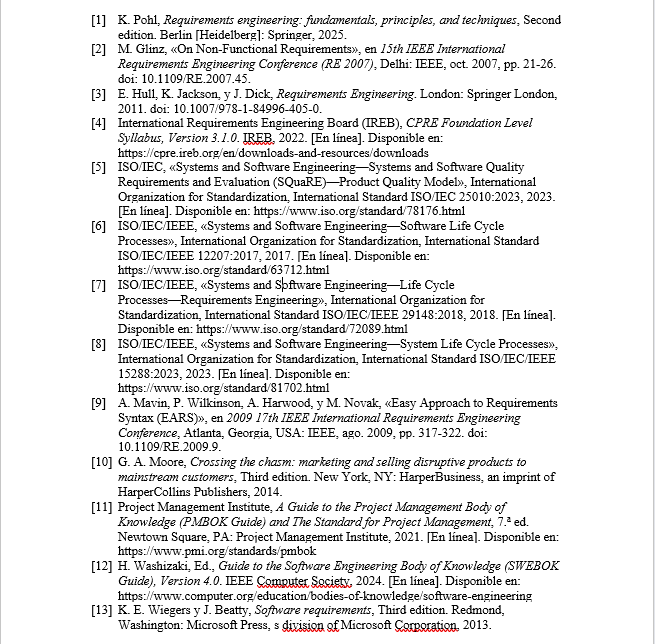
\includegraphics[width=\linewidth,height=0.72\textheight,keepaspectratio]{figura/anexo_a_bibliografia_ieee.png}
}{
\fbox{\parbox[c][6cm][c]{0.87\linewidth}{\centering Captura pendiente de incorporar:\par\texttt{\detokenize{figura/anexo_a_bibliografia_ieee.png}}}}
}
\caption{Salida bibliográfica IEEE de las fuentes principales organizadas por el Investigador A.}
\label{fig:anexo_allan_bibliografia}
\end{figure}

\clearpage
\subsection*{Anexo B. Colección Zotero del Investigador A (Allan)}
\addcontentsline{toc}{subsection}{Anexo B. Colección Zotero de Allan}
La Figura~\ref{fig:anexo_allan_zotero} corresponde a la colección bibliográfica del Investigador A y registra la organización de fuentes principales y complementarias en Zotero. Esta evidencia documental no representa por sí misma la aprobación de los requisitos por los interesados.
\begin{figure}[!htbp]
\centering
\IfFileExists{figura/anexo_b_coleccion_zotero.png}{
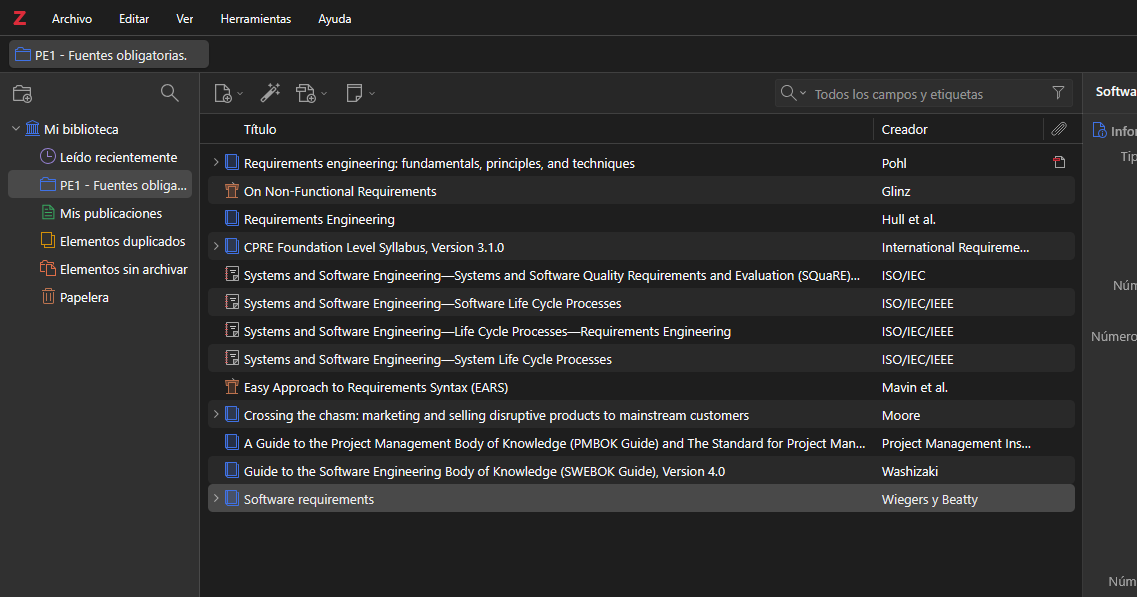
\includegraphics[width=\linewidth,height=0.72\textheight,keepaspectratio]{figura/anexo_b_coleccion_zotero.png}
}{
\fbox{\parbox[c][6cm][c]{0.87\linewidth}{\centering Captura pendiente de incorporar:\par\texttt{\detokenize{figura/anexo_b_coleccion_zotero.png}}}}
}
\caption{Colección Zotero de referencias del Investigador A.}
\label{fig:anexo_allan_zotero}
\end{figure}

\clearpage
\subsection*{Anexo C. Referencias bibliográficas del Investigador B (Freddy)}
\addcontentsline{toc}{subsection}{Anexo C. Referencias bibliográficas de Freddy}
Este anexo recupera la evidencia bibliográfica originalmente identificada como Anexo A en el aporte de Freddy David Rochina Rochina. En el informe grupal se denomina Anexo C para mantener numeración única. La Figura~\ref{fig:anexo_freddy_bibliografia} presenta la salida IEEE de las doce fuentes registradas en su aporte individual.
\begin{figure}[!htbp]
\centering
\IfFileExists{figura/Anexo_A_IEEE.PNG}{
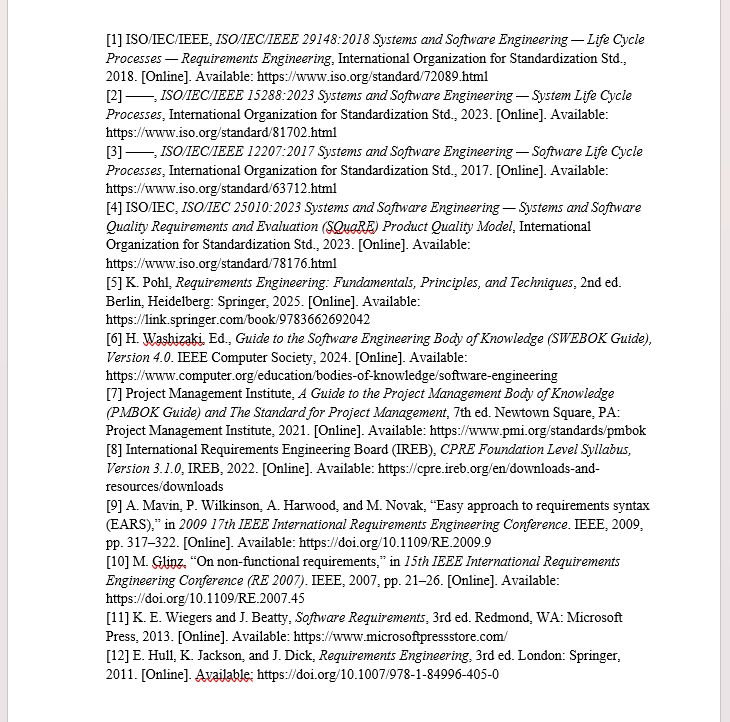
\includegraphics[width=\linewidth,height=0.72\textheight,keepaspectratio]{figura/Anexo_A_IEEE.PNG}
}{
\IfFileExists{figura/Anexo_A_IEEE.png}{
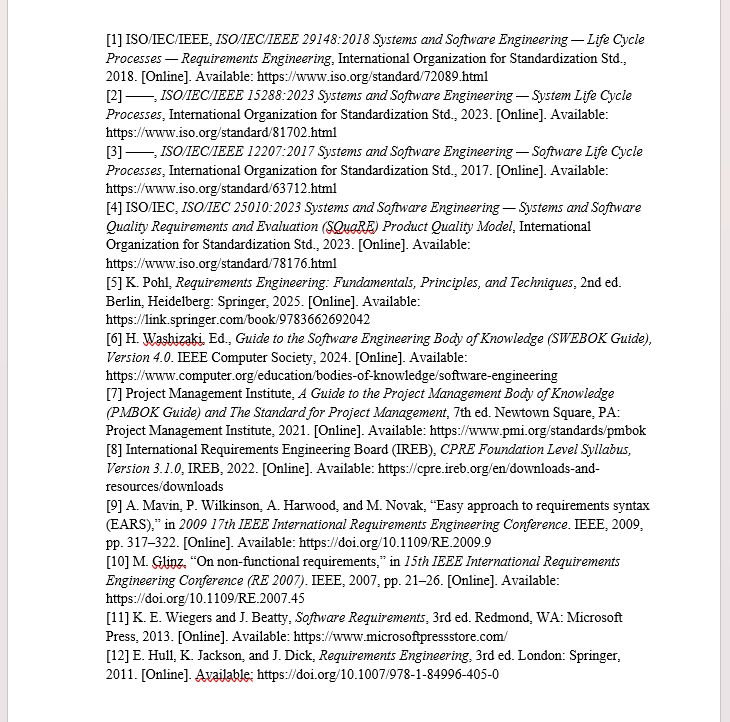
\includegraphics[width=\linewidth,height=0.72\textheight,keepaspectratio]{figura/Anexo_A_IEEE.png}
}{
\fbox{\parbox[c][6cm][c]{0.87\linewidth}{\centering Captura pendiente de incorporar:\par\texttt{\detokenize{figura/Anexo_A_IEEE.PNG}}}}
}}
\caption{Salida bibliográfica IEEE de las doce referencias del aporte del Investigador B.}
\label{fig:anexo_freddy_bibliografia}
\end{figure}

\clearpage
\subsection*{Anexo D. Colección Zotero del Investigador B (Freddy)}
\addcontentsline{toc}{subsection}{Anexo D. Colección Zotero de Freddy}
Este anexo corresponde a la evidencia de colección bibliográfica originalmente identificada como Anexo B en el aporte individual del Investigador B. La Figura~\ref{fig:anexo_freddy_zotero} documenta la organización de dichas referencias en Zotero.
\begin{figure}[!htbp]
\centering
\IfFileExists{figura/Anexo_B_ZOTERO.PNG}{
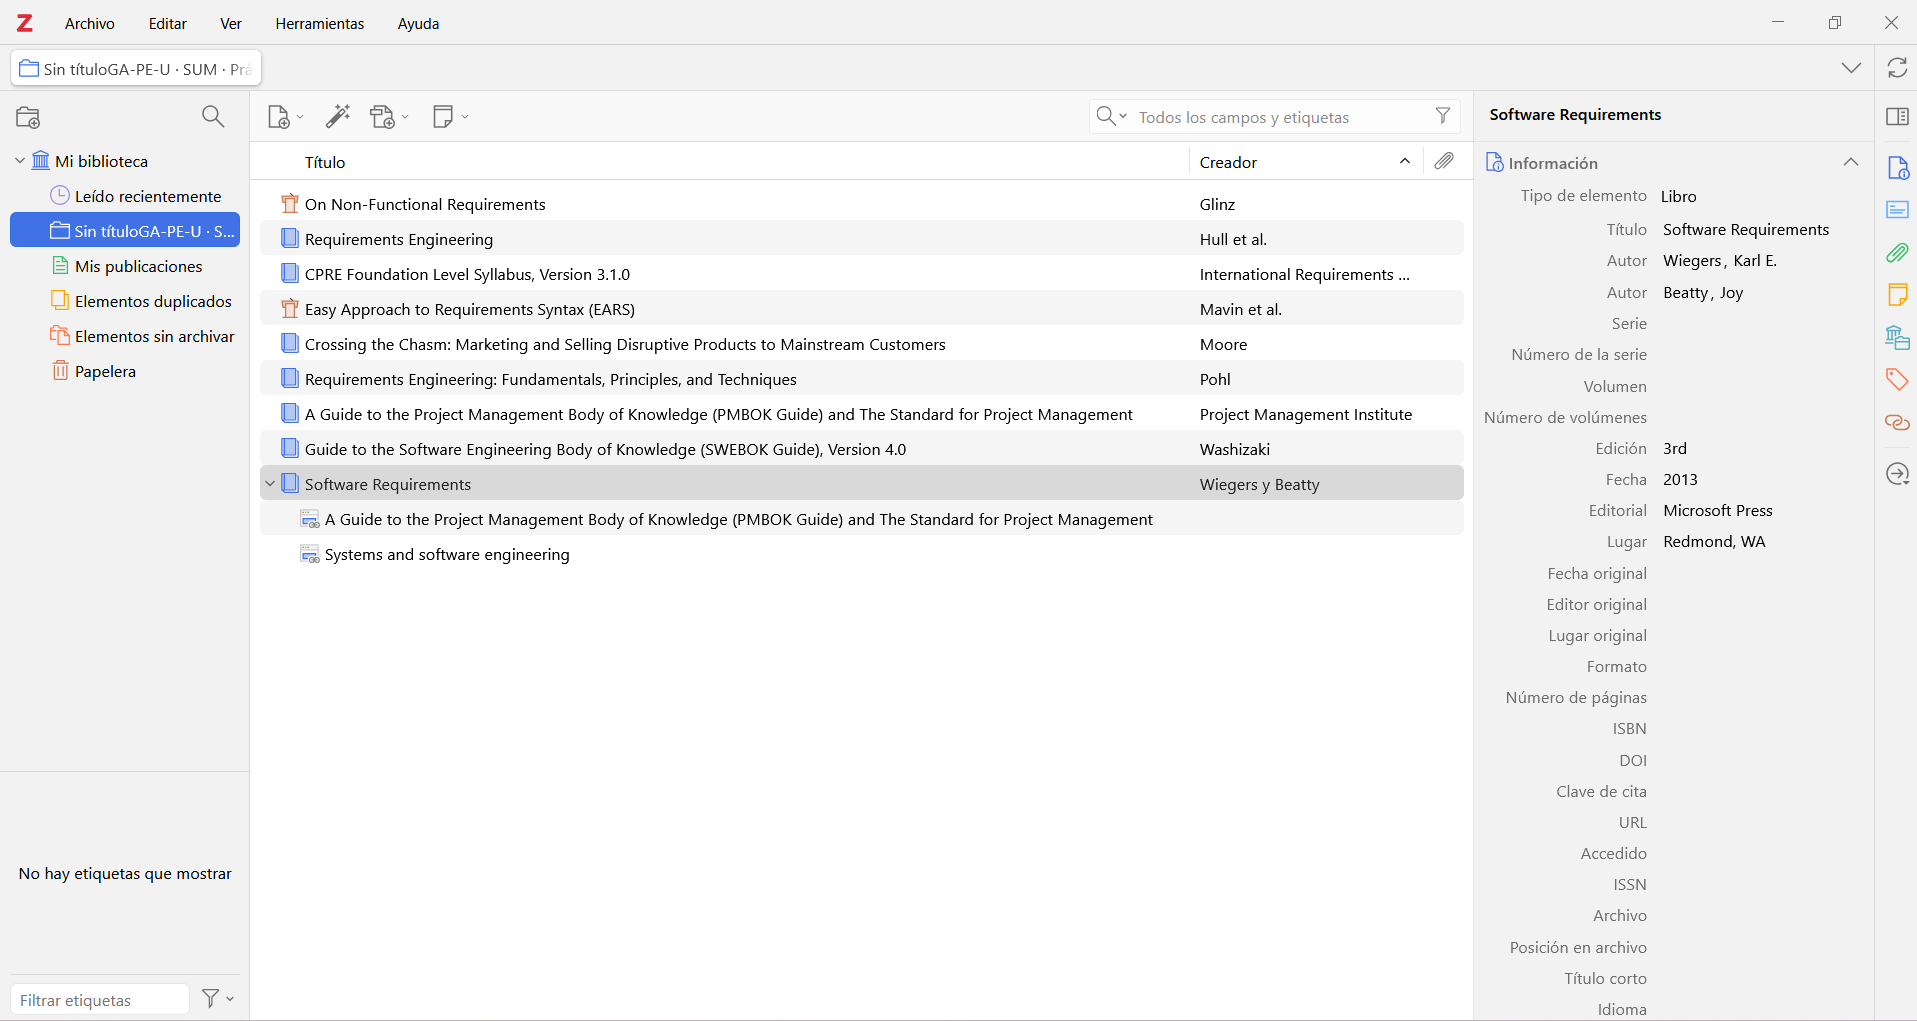
\includegraphics[width=\linewidth,height=0.72\textheight,keepaspectratio]{figura/Anexo_B_ZOTERO.PNG}
}{
\IfFileExists{figura/Anexo_B_ZOTERO.png}{
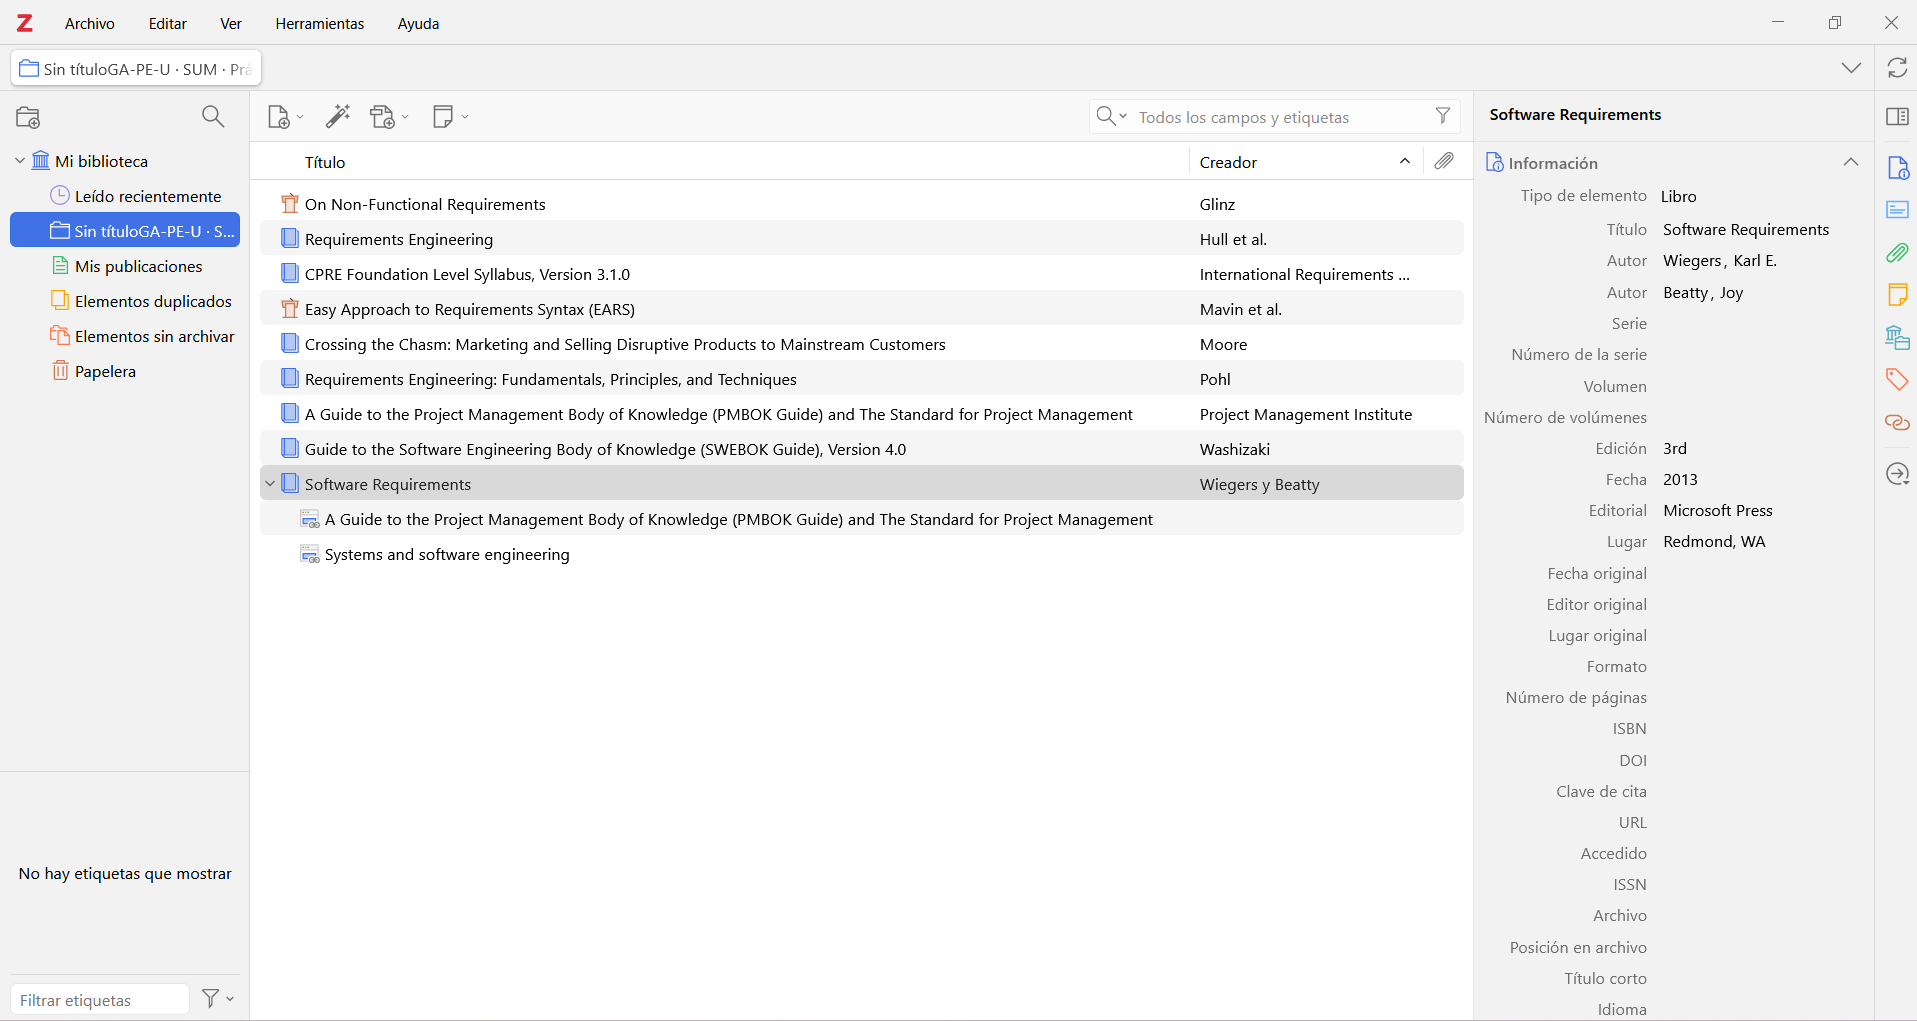
\includegraphics[width=\linewidth,height=0.72\textheight,keepaspectratio]{figura/Anexo_B_ZOTERO.png}
}{
\fbox{\parbox[c][6cm][c]{0.87\linewidth}{\centering Captura pendiente de incorporar:\par\texttt{\detokenize{figura/Anexo_B_ZOTERO.PNG}}}}
}}
\caption{Colección Zotero de referencias del Investigador B.}
\label{fig:anexo_freddy_zotero}
\end{figure}

\clearpage
\section*{Declaración de uso de herramientas de inteligencia artificial}
\addcontentsline{toc}{section}{Declaración de uso de herramientas de inteligencia artificial}
Durante la elaboraci\'on del informe se utiliz\'o ChatGPT como herramienta de apoyo para organizar el contenido, contrastar referencias disponibles, mejorar la redacci\'on y preparar el c\'odigo de integraci\'on en LaTeX. Su intervenci\'on no constituye evidencia de entrevistas, observaciones de campo, aprobaci\'on de requisitos ni ejecuci\'on de pruebas con el establecimiento. La revisi\'on acad\'emica del aporte sobre fundamentos y elicitaci\'on corresponde a Allan Jeremy Mendoza Palma; la de tipos, propiedades y especificaci\'on a Freddy David Rochina Rochina; y la de contexto, actores, l\'imites y perspectivas a Roselyn Andreina S\'anchez Centeno. 
\end{document}